\documentclass[a4paper,12pt,twosides]{book}

\usepackage{graphicx} % to set the title_page image (university's logo)
\usepackage{url}
\usepackage{cite}     % bibliography
\usepackage{geometry} %for margins removal

\usepackage{listings} % makes code look good
\usepackage{color}    % for syntax highlight

\usepackage{pdfpages} % to insert other pdfs  

% these are beeded for the pseudocode
\usepackage{amsmath} 
\usepackage{algorithm}
\usepackage[noend]{algpseudocode}  


\usepackage{fancyvrb} %style verbatim
\usepackage{float} % enforce image positions

\usepackage{afterpage} % to put blank pages after other

\usepackage{csquotes} % to use the right kind of quotes


% this part defines how to do syntax highlight
\definecolor{dkgreen}{rgb}{0,0.6,0}
\definecolor{gray}{rgb}{0.5,0.5,0.5}
\definecolor{mauve}{rgb}{0.58,0,0.82}

\lstset{frame=none,
  aboveskip=0mm,
  belowskip=0mm,
  showstringspaces=false,
  columns=flexible,
  basicstyle={\small\ttfamily},
  numbers=left,
  numberstyle=\tiny\color{gray},
  keywordstyle=\color{blue},
  commentstyle=\color{dkgreen},
  stringstyle=\color{mauve},
  language=Java,
  stepnumber=1,
  numbersep=4pt,
  % breaklines=false,
  % breakatwhitespace=false
  tabsize=2
}
%end syntax highlight

%Automatically add contents
\newcommand\chap[1]{
  \chapter*{#1}
  \addcontentsline{toc}{chapter}{\protect\numberline{}#1}}

%command for blak pages
\newcommand\blankpage{%
  \null
  \thispagestyle{empty}%
  \addtocounter{page}{-1}%
  \newpage}

%center verbatim stuff
\newenvironment{centerverbatim}{%
  \par
  \centering
  \varwidth{\linewidth}%
  \verbatim
}{%
  \endverbatim
  \endvarwidth
  \par
}

\title{DevArtist: a compiler-based approach to application hardening on Android.}
\author{Giovanni De Francesco}

\begin{document}
  \begin{titlepage}
  \pagestyle{empty}

  \begin{center}
    {\bfseries\Large {\huge U}NIVERSIT{\"A}T DES {\huge S}AARLANDES}

    \vspace{0.2cm}

    {\large Department of Computer Science}

    \vspace{0.5cm}

    \begin{center}
      
\includegraphics{img/logo_uds.png}
    \end{center}

    \vspace{0.5cm}

    {\Large Master degree in Computer Science}

    \vspace{0.2cm}
    \line(1,0){338}
    \vspace{0.5cm}

    {\Large Master Thesis}

    \vspace{2.0cm}

    {\Large \bfseries {DevArtist: Evaluating a Compiler-Based Approach to Application Hardening on Android}}

    \vspace{0.3cm}
    

    \large
    \begin{center}
      \begin{tabular}{lcl}
        Supervisor: & \hspace{4cm} &  \hspace{1.5cm} Graduant: \\
        {\bfseries Prof. Dr. Michael Backes} & \hspace{2cm} & {\bfseries Giovanni De Francesco } \\ \\
        Advisor: \\ {\bfseries Oliver Schranz}
      \end{tabular}
    \end{center}
    \vspace{2.0cm}

    {\large \bfseries September, 2017}
    \vfill

  \end{center}

\end{titlepage}

  % \begin{titlepage}
  \pagestyle{empty}

  \begin{center}
    {\bfseries\Large {\huge U}NIVERSITY OF {\huge T}RENTO}

    \vspace{0.2cm}

    {\large Department of Information Engineering and Computer Science}

    \vspace{0.5cm}

    \begin{center}
      
\includegraphics[width=0.3\textwidth]{img/logo_unitn.png}
    \end{center}

    \vspace{0.5cm}

    {\Large Master degree in Computer Science}

    \vspace{0.2cm}
    \line(1,0){338}
    \vspace{0.5cm}

    {\Large Master Thesis}

    \vspace{2.0cm}

    {\Large \bfseries {DevArtist: Evaluating a Compiler-Based Approach to Application Hardening on Android}}

    \vspace{0.3cm}
    

    \large
    \begin{center}
      \begin{tabular}{lcl}
        Supervisor: & \hspace{4cm} &  \hspace{1.5cm} Graduant: \\
        {\bfseries Prof. Dr. Fabio Massacci} & \hspace{2cm} & {\bfseries Giovanni De Francesco } \\ \\
      \end{tabular}
    \end{center}
    \vspace{2.0cm}

    {\large \bfseries Academic year 2016-2017}
    \vfill

  \end{center}

\end{titlepage}

\addtocounter{page}{-1}
\newpage

  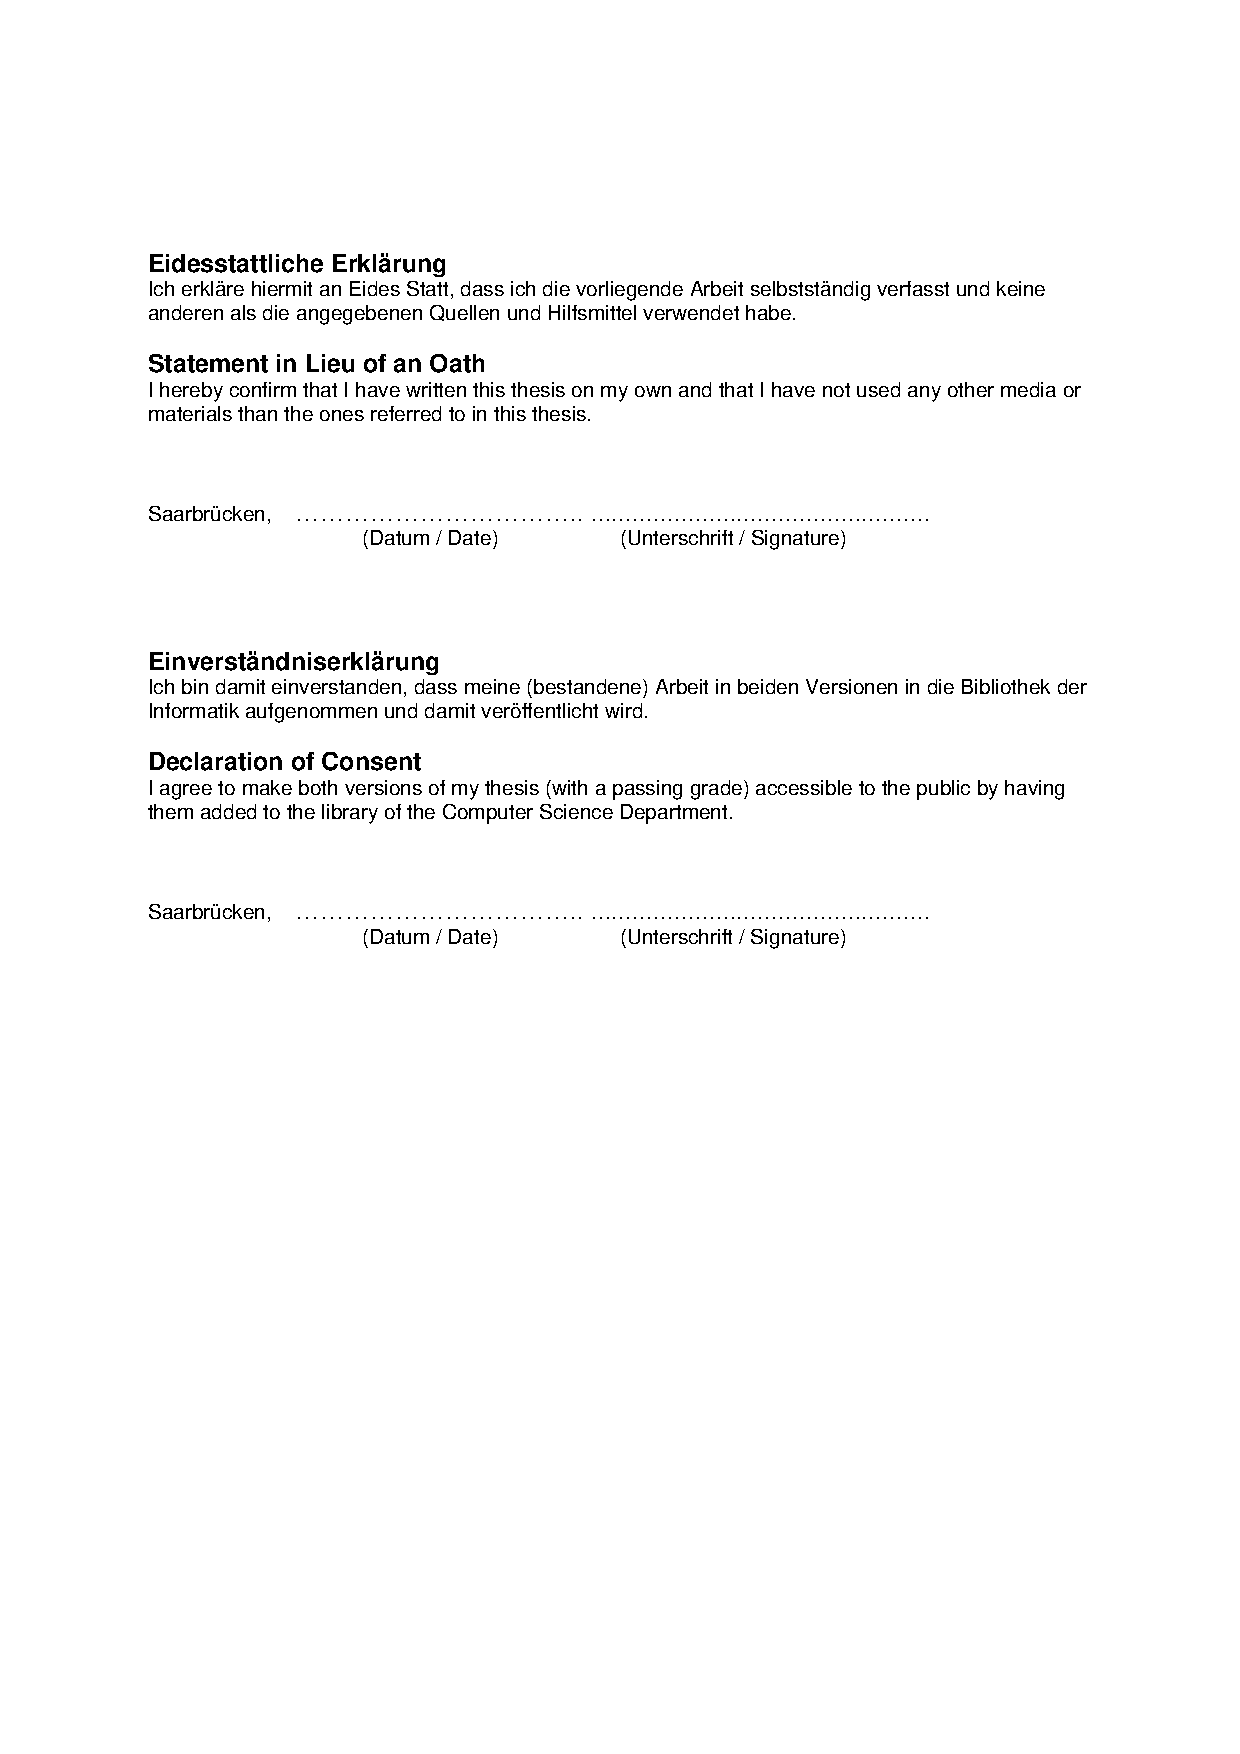
\includepdf[pages={1}]{consent_declaration.pdf}
  \thispagestyle{empty}
\begin{flushright}
\vspace*{3.0cm}
{\large \textit{A mio fratello Emilio,}} \\ 
{\large \textit{piccolo gigante buono.}} \\ 
\end{flushright}

  \frontmatter
  	\tableofcontents
  \mainmatter
    \pagebreak
\hspace{0pt}
\vfill
\textbf{Abstract.}
Android is the most popular mobile Operating System in the world and it dominates the market share, which makes it an important platform for developers to publish applications (apps). Moreover, nowadays, there is an enormous amount of apps available and a part of them is developed by programmers which are not trained to code in a secure manner, leading to user's privacy leakages. Moreover, developers have a hard time finding resources on-line, to avoid common security mistakes. The phenomenon of exploited apps is also growing, despite the effort of Google, which only put in place a layer of automatic testing proved to be insufficient\cite{bouncerfail}. Therefore, we present and evaluate here \emph{DevArtist} a compiler-assisted patching tool for security vulnerabilities. This tool is capable of patching unsafe usage of randomness, sql injections and the usage of obsolete hashing functions such as MD5. Furthermore, it offers an application for end-users to harden their devices and it provides developers a mean to deliver more secure applications. In addition, the implementation of \emph{DevArtist} was analyzed thoroughly with automated testing on real applications already present in the Play Store, to better show its potential and discuss its limitations. In fact, in spite of the prototypical stage of this system, the evaluation suggests that such a tool reduces the exploitable attack surface of apps, which leads to less privacy leaks, hence aiding in the battle against Android malware.
\vfill
\hspace{0pt}
\pagebreak

    \chapter{Introduction}
In both 2016 and 2017, many major anti-virus companies and Nokia, showed in their security reports how the Android mobile Operating System was the most targeted platform\cite{kaspersky}\cite{mcafee}\cite{nokia}: the reason behind such a great focus on this platform becomes clear when that information is used in combination with the market share data provided by the International Data Corporation. In fact, in the third quarter of 2016, Google's Operating System (OS) was running more than the 85\% of the smart-phones worldwide\cite{idcshare}. Moreover, based on the above-mentioned reports, the majority of devices gets infected by downloading a tainted app from the Play Store, despite Google's efforts to keep it a safe zone by leveraging many layers of automated testing. Furthermore, this is a problem which burdens especially those security-focused environments where devices need to run trusted software and administrators cannot even allow their users to download applications from the main store. In the next sections and chapters, I will investigate what is needed to tackle the problem of hardening Android applications, offering a compiler-based approach to find and patch common vulnerabilities, but even more importantly, evaluating if this solution could be an important asset in the fight against malware on the Android Ecosystem.

\section{Motivations}
Bug discovery and patching is an important part of every development cycle: the goal is always to produce a robust and reliable application for end users, especially for security-oriented ones. However, this process requires time and the modern market for mobile apps\footnote{short for applications}, moves at a tremendous speed, requiring companies to release software fast enough to not be out-sped by competitors. In parallel to this problem, the Android Operating System evolves constantly and, not only Google introduces new APIs in every version, but the entire ecosystem flourishes with new libraries, extensions and forks which get released everyday.
Keeping up with all this novelty can be cumbersome both for developers themselves, but also for companies which would like to provide up-to-date courses to others on how to write secure code. Moreover, Google provides only one page of security tips to programmers\footnote{\url{https://developer.android.com/training/articles/security-tips.html}}, but its worth to note that there is not a single line of code in the whole page and, even though it provides insights on where security holes might happen,  it leaves the task of figuring out how to avoid the described problems to the reader. In addition, developers are not helped in this regard when they are looking for information on the Internet: a quick search on how to solve \texttt{HTTPS} related problems, when making requests with Android, produces results on Stack-Overflow where the most up-voted answers tells to accept any kind of certificate for any given URL, as showed in \cite{svm-hunter}. Another example: when a developer looks on the Internet how to execute the sql \texttt{SELECT} statement on Android: the most up-voted answers claim that you need to use the \texttt{rawQuery} method which is subject to SQL Injections, as explained a few pages further. However, the most compelling argument for this work was given by the result of an automated investigation which I conducted on Android apps published on the Play Store. In fact, given all the problems described above, I assumed that most applications would be vulnerable to well known attacks and the results, as described in the evaluation chapter, were indicating that the hypothesis was correct and they also hinted at the necessity of this work. 

\section{Contributions of this Work} 
Since the first public release of the Android source code, which was made in April 2009\footnote{\url{https://developer.android.com/about/versions/android-1.5-highlights.html}}, tools such as CHEX\cite{chex}, DroidAlarm\cite{droidalarm} and the more recent AppoScopy\cite{apposcopy} provided means to perform static analysis and, on the other hand, AppsPlayground\cite{appsplayground} and AspectDroid\cite{AspectDroid} offered only ways to use dynamic analysis. The only tool which really patches common vulnerabilities is, as the name suggests, PatchDroid\cite{patchdroid}. However, its focus on back-porting patches to old devices for privilege escalation attacks and its reliance on the Dalvik byte-code made it cumbersome to use since Android 5 Lollipop, when ART and its on-device compilation was introduced. Therefore, there is a need for a tool which can fill the gap that PatchDroid left on newer devices. The contribution of this thesis started by studying this need and by creating a prototype for it, namely DevArtist, which aim is to patch common security vulnerabilities by leveraging Android's ART runtime. Given the novelty of compiler-assisted patching tools, this work contributes also in evaluating this approach.

\section{Outline}
The structure of this work is as follows: knowledge about Android, ART and Information Flow control are introduced in the second chapter together with a primer on \emph{Artist} and its front-end \emph{ArtistGUI}. The third chapter discusses already existing research and how this work differentiates from it. The fourth chapter provides the need of this work: introducing the problems which \emph{DevArtist} solves and evaluating their severity. Chapter five describes the prototype produced for this thesis: it provides information about the design of such system and explains the algorithms developed. Furthermore, Chapter six shows how the evaluation of \emph{DevArtist} was conducted and presents its result. 
Finally, Chapter eight draws the conclusions of this work after chapter seven has discussed what future development paths might be.


    \chapter{Background Knowledge}
\label{ch:background}
To understand the chapters ahead and ease the reader into this work, here are defined all the required notions on which DevArtist and its evaluation rely on. In addition, this chapter offers the necessary terminology and a place to reference later in the thesis. For obvious reasons, all the information provided here will be focused on Android but, where possible, attempts to provide the general idea are made.

\section{Android Architecture}
Android can be seen as a heavily customized Linux distribution, where Andy Rubin and his team, the original developers of Android, implemented a set of features and a UI framework with the goal to target mobile devices. Sharing the kernel with other distributions makes it easier for hardware companies to write drivers and enables Android to use a multitude of already existing C/C++ libraries which have been developed and tested through the years. In addition, the OS also abstracts those libraries and allows application developers to make use of them through a Java API: the Android SDK. A simplified version of the Android software stack is reported in Fig: \ref{fig:androidstack}, a full version of its documentation is available in \cite{and_doc_stack}.

\begin{figure}
	\centering
	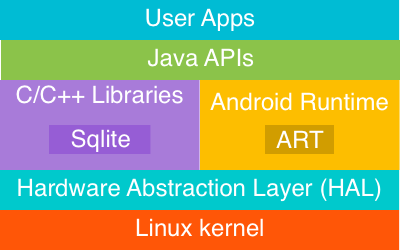
\includegraphics[scale=0.8]{img/android_stack.png}
	\caption{Android Platform Overview\cite{artist}}
	\label{fig:androidstack}
\end{figure}

\section{Android's Application Package}
Any Android developer can develop apps through the Android SDK provided by Google. The main language is Java but it's also possible to use the Android NDK and develop in C/C++, even though it's not suggested. At the moment of writing also Kotlin, a language that compiles to JVM byte-code, is officially supported and it is gaining momentum. Moreover, when an app is ready, its code gets compiled through the \texttt{javac}  compiler and \texttt{dx} tool, which transforms all the \emph{.class} files into one or more\emph{.dex} files, which are compatible with the Dalvik Virtual Machine (DVM). Successively, the produced byte-code is compressed together with other files, such as the Manifest and developer signature, forming Android's Application Package (APK).

\section{Android Internals}
The following subsections offer information about one service and one API, which are provided by the OS and are important because mentioned throughout this thesis.

\subsection{The Logcat}
On Android, there is no standard output and every call to the \texttt{System.out.println} (depending on the implementation by the device manufacturer) gets redirected by the OS to the default logging system. This system can be used by developers through the \texttt{Log} class and it provides five main channels for messages: ERROR, WARN, INFO, DEBUG and VERBOSE, which respectively are used to report the right kind of information. Moreover, all the log messages produced by both the OS and developers can be analyzed through the Logcat program, which is shipped within the Android Debug Bridge (ADB, a collection of development programs for Android) and integrated in both Android Studio and Eclipse.

\subsection{Public Components}
\label{sc:exportedcomponents}
Among the primary building blocks of the Android ecosystem, there are re-usable components: specific parts of an application's code which also can be used by other applications installed on a device. The goal of such a system is to provide developers a way to make use of data and computation of other apps without the need to manually gather the information or code an extra functionality. An example of this behavior can be found every time an application, such as Evernote, needs to save an appointment: it can open the default calendar application and let the UI of this latter application handle the appointment creation and sync with a server. Another example might be a medical application which lists all the checks that a patient needs to attend to: in this case, it can ask the calendar application to provide all the appointments with the flag \enquote{medical} or \enquote{Dr.} and display them without actually managing the data. The system also prevents that different applications alienate the user with different UIs for the same task, providing better consistency across the platform. However, this components might be dangerous from a privacy standpoint, due to the fact that, through them, applications which do not have permissions to view sensitive information, instead, gather access to it. For this reason, the developers of the Android SDK limited this functionality only to four main components: Activities, Services, Content Providers and Broadcast Receivers, which all can be used as entry-points for an application and accessed through different mechanisms. In particular Content Providers, which this thesis focus on, can be accessed from outside the application by adding the flag: \texttt{exported="true"} to its declaration in the Manifest file. Unfortunately, the SDK does not provide any security measure to restrict these exported components to a subset of apps besides the one signed with the same signature (which in part voids their goal), leaving the job to application developers. 


\section{Application Analysis}
There are many kinds of automated analysis, which can be performed on programs and, consequently, on mobile applications. The sub-genre, on which we focus, is letting another program perform an inquiry on the security of an arbitrary application. Moreover, this kind of examination branches in two separate directions, depending at which level of the software is executed, specifically: static analysis works on the source code or byte-code level of an application, whilst dynamic analysis is computed at runtime. There are advantages and disadvantages in both of them, although our system, as many others, combines them in order to achieve better accuracy.
It would be easy to think that instrumenting Android applications could be simple enough and that any tool developed for GNU/Linux up to now could be used, as also done by Min Zheng et al in DroidTrace\cite{droidtrace}, where they leveraged \emph{ptrace} to perform dynamic analysis. However, this is not the case due to the fact that this technique allows to perform the analysis only on the lowest part of the Android software stack, precisely the kernel system calls, leaving open the analysis at the level of Java APIs. 

\section{Application Instrumentation}
Instrumenting an application fundamentally means extending static or dynamic analysis to the point of changing or extending its behavior. In fact, popular uses of instrumentation are: code-tracing, profiling and even debugging. Instrumentation also is sub-divided in two branches and its named source instrumentation the one which operates at the source code or byte-code level, while the name binary instrumentation is used whenever the changes apply at the executable level. The most common way to instrument applications is via hooking specific parts of the code and then call another one, implemented separately, whenever that point is reached. This technique, used jointly with Inline Reference Monitoring (IRM)\cite{irm}, has been modified and employed on Android by quite a few researchers. In fact, as shown by AspectDroid\cite{AspectDroid}, CHEX\cite{chex} and others, this technique is still valid and allows to hook Android application's byte-code. However, on this OS, this approach also requires re-packaging, which consists in extracting all the code and resources from one apk to copy them into a new one with the changes needed to hook. Moreover, for security reasons, the Android system requires each apk to be signed and, since the original key is known only to the app's developer, the approach must include another signature. Signing with a different key breaks application updates for users though, since the Play Store uses it to verify apks. Therefore, this thesis aims to keep these possibilities for the user and base its novelty on the new approach provided by the Android Runtime.


\section{Android Runtime}
The Android Runtime (ART) introduced ahead-of-time compilation (AOT) since Android 4.4 and made it the default on Android 5, definitely replacing  the DVM. This change did not only improve app performance, but also required a shorter app installation time. However, changing the way applications are compiled and executed could have meant significant losses in the amount of already published apps on the store because of incompatibility with the new system. Therefore, Google's engineers maintained the compatibility with the DEX file format by using an on-device compiler called \textbf{dex2oat}, which takes the Dalvik code (dex code) and transpiles it to native machine code. Due to the nature of Android, this compiler is greatly modularized and it is capable of generating native code for a multitude of architectures, such as: mips, mips64, x86, x64, arm and arm64. In particular, dex2oat defines three backends: \emph{Quick}, \emph{Portable} and \emph{Optimizing}, all of them specify a different behavior regarding how the dex code is handled. However, since the first is strictly derived from the DVM and the future of the second is uncertain\cite{artist}, in this thesis we focus more on the latter. 

\subsection{Optimizing Backend}
This backend option became the default for app compilation since the release of Android 6 Marshmallow, dropping the \emph{Quick} one almost completely, which is now only used to compile Android's boot image. The main reason for this change was that \emph{Optimizing} allowed state-of-the-art code optimization techniques such as the removal of: dead code, redundant bound check or even duplicate code. In particular, this backend defines a structure for developers to create optimization steps that work on the Intermediate Representation (IR) of the dex code contained in the APK file.

\subsubsection{Intermediate Representation}
ART's AOT compilation, as many other compilers, uses an Intermediate Representation (IR) before transforming dex code to machine code. In fact, the main role of dex2oat can be summarized as creating the IR from the dex code and then performing optimization steps on it. Moreover, the IR of a program can be seen as an oriented graph, where every instruction scanned from the beginning of the dex code represents a node. This particular form of this graph is called Control Flow Graph (CFG) because it maps every flow of the code, showing not only where it branches but also why. Specifically to the IR used by dex2oat, the instructions are reduced to single static assignment form (SSA), which is ensuring that every variable is assigned exactly once and they can be represented as a string having the following structure:
\begin{figure}[H]
\centering
\begin{BVerbatim}
instruction_id: instruction_type:method_name(inputs)[uses]
\end{BVerbatim}
\end{figure}
where the id is given by the compiler, the types are either: ParamValue (a parameter passed to a function), basic mathematical operations (add, xor, and, etc...) or the type of method which is invoked. However, there are many more types of instruction which this work does not analyze and they can be found in \cite{artist}. Furthermore, \emph{inputs} is a comma separated list of all the arguments that need to be passed into the method, whilst the \emph{uses} are also a comma separated list of all the other instructions, where that method is then used later in the code. Table \ref{tab:exampleAdd} offers an example of conversion from Java code to the IR.\newline

\begin{table}[h!]
  \centering
  \begin{tabular}{|c|}
  	\hline
	\begin{lstlisting}[language=Java]
	public int getRandomNumber(long seed){
		Random rnd = new Random(seed);
		return rnd.nextInt();
	}
	\end{lstlisting}\\
	\hline
	\begin{lstlisting}[language={[x86masm]Assembler}]
		getRandomNumber: Basic block 0
		0: ParamValue(this)
		1: ParamValue(Long)[3]
		2: newInstance:java.util.Random()[3]
		3: InvokeStaticOrDirect:java.util.Random<init>(1)[3]
		4: NullCheck(2)[5]
		5: InvokeVirtual:java.util.Random.nextInt(4)[6]
		6: Return(5)
	\end{lstlisting} \\
	\hline
  \end{tabular}
    \caption{Java code on the upper side, IR representation on the lower one}
	\label{tab:exampleAdd}
\end{table}

\subsection{The Special Case of NullCheck}
In order to avoid accessing null objects at runtime and throw a \texttt{NullpointerException}, the compiler inserts a special instruction before every method of an object instance gets called, which has type: \texttt{NullCheck}. As it can be also seen in Table \ref{tab:exampleAdd}, this instruction always has as it's first input a reference to instruction which contains the instantiation of the object upon which the null check has to be computed. This property will come handy to compute backward slicing later in this work.


\section{Program Slicing}
An entire branch of Computer Science is dedicated to the field of Information Flow Control (IFC), which studies how data is passed and transformed by processes. In particular, especially in the security field, it is important to track the mutations of variables, to prevent data leaks and other privacy issues. Therefore, to achieve this goal, Reps and Yung introduce in \cite{slicing} the concept of program slicing and they define what is the \emph{Backward} and \emph{Forward} slice of a line of code, abbreviated in BS(x) and FS(x), but also, they prove formally that the BS(x) contains all the operations which influence a line of code x. In fact, the BS(x) is the collection of all the previous lines of code that cause a change to x, whilst FS(x) is the collection of all the lines of code that follows x, which change when x does. Moreover, inside the BS(x) we can define a Source (So), which is the line where the tracked data is first defined, and a Sink (Si), which is the last usage of that data. Table \ref{tab:slicing} shows an example of slicing where the source is line 2 and sink is line 5, please mind that a sink can also be a return operation and not only an output operation. However, although the example shows slicing on Java code, slicing is the core of the optimizations steps performed on  IR by the Optimization backend and, consequently, Artist.    

\lstset{numbers=none}
\begin{table}[h!]
  \centering
  \begin{tabular}{|c|c|}
  	\hline
	\begin{lstlisting}[language=Java]
	public void Print10Bar(int n){
		int x = 10;
		bar(x+n);
		x++;
		System.out.println(x);
	}
	\end{lstlisting} &
	\begin{lstlisting}[language=Java]
		int x = 10;
		x++;
		System.out.println(x);
	\end{lstlisting} \\
	\hline
  \end{tabular}
    \caption{Java code on the left side, BS(5) on the right}
	\label{tab:slicing}
\end{table}


\section{Artist and ArtistGUI}
Artist is a new Android instrumentation framework for security researchers and developers which stands on top of dex2oat's optimizing backend. It is composed of a static and a dynamic component: the first one is able to instrument the application at compile time, whilst the other is a library merged into the app. This method not only allows for better instrumentation but has serious advantages for the user, who can keep updating the application as they used to.

\subsection{Artist}
\label{sec:artist}
ART Optimizing backend implements a few optimization steps, which already work on the IR graph. Hence, the developers of \emph{Artist} implemented it as a new optimization step, which is able to compute CRUD\footnote{Acronym for : Create, Read, Update, Delete} operations upon the IR, thus achieving static analysis and source instrumentation. Moreover, it enables third-party developers to hook the right instruction target(s) by implementing a visitor pattern on the IR graph, and then, it exposes helper methods which can replace, modify, move or even delete the chosen instruction(s). In this way, when the compilation actually happens, the resulting native code reflects the modified IR graph (IR*) and not the original one, thus allowing the change of behavior in the app. Figure \ref{fig:optbackend} provides a visual representation of the work-flow inside the newly changed Optimizing backend of dex2oat and helps in creating a mental map of the steps involved in the process.

\begin{figure}[H]
	\centering
	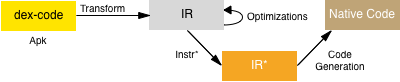
\includegraphics{img/dex2oat.png}
	\caption{The optimizing backend with Artist}
	\label{fig:optbackend}
\end{figure}

\subsection{ArtistGUI}
The dynamic analysis is provided by an Android app called ArtistGUI, which includes the dex2oat binary and enables the end-user to compile apps with it. Instead of statically linking the compiler, this app uses the \texttt{LD\_LIBRARY\_PATH} directive to ensure that all the libraries needed by dex2oat are loaded. Furthermore, the app shows a list of already installed apps and, when one is tapped on, it performs two main functions: first it merges an auxiliary library into the app and then it re-compiles the chosen app with its own dex2oat. The afore-mentioned library is also produced by the developer that creates the Artist module and it is often used both to perform the analysis of the app at runtime but also to aid the insertion of new instructions in the IR at compile level. In fact, since creating new code on the Artist side is hard due to its representation, developers can create this code in Java within the library and then insert them at the compiler level whenever they need by referencing it.

\begin{figure}[H]
	\centering
	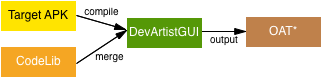
\includegraphics{img/devartistgui.png}
	\caption{The work-flow of ArtistGUI}
	\label{fig:installprocess}
\end{figure}

\section{Automated Testing}
Proving the need and the soundness of this work would have required too much time if executed manually, due to the fact that it had to be tested on real apps. Therefore, layers of automated testing has been set up, not only to download applications from the Google Play Store but also to instrument, check their behavior and automatically generate a full report, which can be manually analyzed to extract important information.

\subsection{Monkey Troop}
The developers of \emph{Artist} also provide \emph{Monkey Troop}, a python tool which can automatically test an \emph{Artist} module. This system is capable of installing applications, run them, tap on the screen as an user would do and instrument them with a specified module. It also generates a report, with the full Logcat (Android's standard output log) for each application. Unfortunately, the tool comes with little documentation, which is available with the code on Github \cite{monkeytroop}. However, the steps to use Monkey Troop are limited to defining a list of links to apps on the Play Store and creating a set of commands, which the system has to execute on a target device to successfully test the module. The device must already have the front-end of the module (ArtistGUI) installed and the tool automatically uses it to instrument every application on the above mentioned list.

\begin{figure}[H]
	\centering
	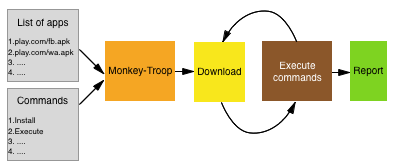
\includegraphics{img/monkey_troop.png}
	\caption{Monkey Troop Overview}
	\label{fig:monkeyoverview}
\end{figure}


     \chapter{Related Work}
During the course of the years, many researchers made efforts in the fight against malware on Android and it is important to contextualize where \emph{DevArtist} places itself among existing solutions. Therefore, this chapter presents previous work on instrumentation of Android applications and/or their patching, discusses how they improve the \emph{state-of-the-art} and how they relate to this work.

\section{PatchDroid}
The most prominent tool in existing literature about patching security vulnerabilities on Android is \emph{PatchDroid}\cite{patchdroid}. Due to the OS fragmentation, this tool focuses on delivering security patches to older Android Devices, which are not updated anymore by the manufacturer. Mulliner et al, provide an Android application which is able to download, from a trusted repository, patches and apply them trough a daemon. In particular, this daemon computes the check of which patch to apply to which processes and is able to patch both native code and Dalvik byte-code.
Native code is replaced by a secure version by Inline Hooking or by hooking the Global Offset Table, whilst Dalvik Code instead is patched by hooking common system calls, such as \texttt{epoll\_wait()}, and replaced with a secure native one through the Dalvik JNI bridge. Moreover, the main functionality of PatchDroid can be also achieved by our system, as discussed in chapter \ref{ch:futurework}.

\section{CHEX}
This static vetting tool, is capable of detecting component hijacking and data leakages within an application. To achieve this goal, the authors define a set of common policies for leakages and, after the tool creates it from the Dalvik byte-code, the complete data-flow graph is checked against those policies to detect leakages. The most clarifying example Lu et all\cite{chex} make to explain the capabilities of the system is when the location of the user is sent through the network. In the example, CHEX is able to recognize that the policy: \enquote{Sensible Source ends in public output} is not respected and prevents the leakage. The functionalities provided by CHEX are also provided in prototypical form by \emph{TaintArtist} (a module inside \emph{Artist} itself), as stated in \cite{artist}, which started as a taint analysis tool. Therefore, our system includes and benefits from this research.

\section{FlowDroid}
In \cite{flowdroid}, Arzt et al. present the first static analyzer tool aware of the Android App's life-cycle and UI widgets. In fact, the asynchronous paradigm adopted by Android apps had limited immensely static analyzer tools up to that point. Therefore, FlowDroid extends what CHEX already did and manages to detect even more leakages from callbacks triggered by the Android Framework. In addition, in this paper also \emph{DroidBench} is presented: a micro benchmarking suite for Android flow analysis. In particular, this is a collection of 39 hand-crafted applications specifically created to be analyzed by static and dynamic tools. In this regard, \emph{TaintArtist} has been tested against the \emph{DroidBench} suite, making also \emph{DevArtist} benefit from this benchmarks. However, FlowDroid, in its current state can only detect but not patch those security leakages.

\section{EPICC and SIFTA}
Both EPICC\cite{epicc} and SIFTA\cite{sifta}, are evolutions of the above mentioned FlowDroid and their aim is to detect leakages on a broader scale. The first is able to detect privacy leaks happening when Inter Components Communication (ICC) is involved between more apps. In fact, it can create a data flow graph (from the Dalvik byte-code), which includes leaks in public components (exported, in Android) such as Intent Filters, Services, Receivers and all the others. SIFTA pushes the state of the art further by using FlowDroid and EPICC on all the installed apps as its first phase, but then, it uses their resulting graphs to create an even greater graph which includes all those applications. Unfortunately, the current state of \emph{TaintArtist} does not allow taint tracking across apps but, it can be achieved if both apps are also instrumented.

% \section{Static Analysis}
% Most of the research int his field focuses in detecting whether an app is malicious. In fact, static analyzers for Android are the first line of defense against malicious apps, due to the fact that their execution can be started directly when the apk is uploaded into the Play Store to detect anomalies in their behavior and block their proliferation before they are even downloaded from final users. Therefore, at the beginning of the research, projects such as Dare\cite{dare} aimed to re-target DVM byte-code to the correspondent Java byte-code, allowing the usage of all already available Java static analysis tools, but for Android apps. Afterwards, systems like CHEX\cite{chex} and Apposcopy\cite{apposcopy} were developed to specifically target Android apps, focusing more on privacy leaks generated from single components (exported Services and Content Providers) or to detect exploits similar to the \emph{GoldDream}\cite{golddream} malware family. Moreover, their strategy was based on the Dalvik byte-code because they were released before  Android 4.4 (KitKat). Only later, FlowDroid\cite{flowdroid} brought also the DroidBench benchmark suite, consisting of a multitude of test cases to assess the soundness and precision of static taint tracking approaches, which became practically the standard suite to test static analysis techniques. In fact, these tests were then re-used by systems such as Amandroid\cite{amandroid} and Iccta\cite{iccta}, which pushed forward the \emph{state-of-the-art} by enabling Inter-Component Communication (ICC) static analysis and also \emph{Artist}\cite{artist} was benchmarked with the above mentioned suite. Recently, the whole research above was even further extended by SIFTA\cite{sifta} which combines Flowdroid and EPICC\cite{EPICC} in its first phase to analyze single apps and then , in its second phase, constructs an \emph{inter-apps} graph by combining their information. Once the graph is ready, SIFTA can perform static analysis and detect leakages.\newline\newline
% \emph{DevArtist} is inherently different to the already presented static analyzers, due to its focus on patching. As a matter of fact, \emph{DevArtist} can not detect any information leakage or families of malware, but it can detect and patch specific and exploitable vulnerabilities. For this reason, it's not advisable to use \emph{DevArtist} as a tool to enforce security standards on apps of the play store as soon as they are uploaded.

% \section{Dynamic Analysis}
% The goal of dynamic analysis on Android aims to defend end users when a malicious app is already installed in the system. The research began with DroidTrace\cite{droidtrace}, which re-used the already existing Linux solution called\texttt{ptrace} to hook into system calls and trace them, preventing unwanted leakages. Afterwards, TaintDroid \cite{taintdroid} became the most used project due to the fact that it wasn't limited to system-calls, but it instruments directly the Android DVM to track information leakages in apps. However, the limit of this system were showed later with ScrubDroid(or AntiTaintDroid) by Sarwar et al in \cite{antitaintdroid}, when they managed to leak sensible private data such as the IMEI and the Android ID over the network without letting TaintDroid know.\newline\newline
% \emph{DevArtist}, again, differentiate itself from the above method dynamic analyzers because it doesn't detect when a private information is leaked at runtime, but it leverage the information available during execution to avoid the usage of insecure method calls or tainted variables. Moreover, \emph{Artist} is the first dynamic system which uses ART instead of DVM, which is now not in use, thus making TaintDroid not functional anymore.

% \section{Information Flow Control}
% As already mentioned in Chapter \ref{ch:background}, one of the fundamentals on which IFC stands is the concept of Program Slicing, published in \cite{slicing} by Reps and Yang. This concepts allows to reduce the execution path only to the important parts, thus allowing speed improvements in the analysis of programs and the study of taint variables directly derives from it.\newline\newline 
% //TODO check with Oliver if this section is needed and in case expand it\newline\newline
% Of this particular field, \emph{DevArtist} relies heavily on the concepts of Backward and Forward Slice to perform its computations, but it does not improve the \emph{state-of-the-art} in any way.

% \section{Compiler-Based Instrumentation}
% Beside \emph{Artist} (hence DevArtist), LLVM was also a major platform for compiler-assisted instrumentation, which allowed writing extension of the compiler thanks to its LLVM-Pass technology\cite{llvmpass}. In fact, project such as LLCov \footnote{\url{https://github.com/choller/LLCov}}, which is used for better code testing coverage, or LDC \footnote{\url{https://wiki.dlang.org/LDC_LLVM_profiling_instrumentation}} for profiling. However, not many projects on LLVM focus on security, with the exception of: AFL/LLVM\footnote{\url{https://github.com/mirrorer/afl/tree/master/llvm_mode}}, which is an LLVM implementation of the AFL Fuzzer, and "pa.llvm"\footnote{\url{https://github.com/codelion/pa.llvm}}, which (in theory) is able to perform dynamic taint analysis. However, all the projects are available only on GitHub, with scarce documentation and no peer-reviewed paper to support them.\newline\newline

% \emph{DevArtist} manages to be easier to use than any other compiler-assisted instrumentation, due to the fact that: in one hand, it does not require the developer to re-compile the program manually but it allows to use its application to check for the vulnerabilities, and in the other hand, it can be used by the final user without knowing anything that stands behind it.
    \chapter{Preliminary Investigation}
\label{ch:investigation}
One of the most recurrent subject in talks regarding Android, is how much the platform does not help developers write secure code. Speakers usually make examples of how developers forget to make usage of private mode when saving preferences or either resorting in saving important documents on the SD card, where are publicly available\cite{codemotion}. Moreover, resources such as Stack Overflow\footnote{\url{www.stackoverflow.com}}, where developers can share solutions to common problems, do not really help when the security of the published code is often of no importance. Therefore, before starting this work, I identified common vulnerabilities which I thought could be fixed at the compiler level and each of them is here presented with an appropriate threat model\footnote{To prevent malicious uses of this work, threat models are explained in as much details as possible, but no code will be provided.}. Furthermore, the fact that these problems were reported did not mean that they were present in top Android apps, hence, before actually creating \emph{DevArtist} to solve these security issues, an investigation was necessary to determine whether they were present and how wide-spread they were.

\section{Hashing}
The term is used to identify the process of transforming data of arbitrary length to data of fixed size, which can be obtained with so called \emph{Hash functions}. Many fields of computer science use these functions to achieve a variety of results, ranging from memory optimization to algorithms which produce randomness or, as analyzed in this thesis, to verify data integrity. However, the possibility to use such functions in the latter field, exists due to another property: collision-resistance. In fact, any secure hash function is collision-resistant in the sense that it is computationally hard to find two inputs which produce the same hash, otherwise it is said that such function is not cryptographically secure in respect to collisions. Furthermore, due to the fact that on Android the full Java cryptography package is available, a developer must decide which hashing algorithm has to use, depending on its use case because not all of the already existing ones are cryptographically secure.

\subsection{The MD5 Case}
Message Digest 5, hence the MD5 acronym, was developed by Ronald Rivest in 1991 and it was formalized on RFC 1321. However, since Dobbertin found a collision\cite{dobbertin} in 1996, many other publications reported cases against the algorithm, culminating in 2012 with Marc Stevens, who published in \cite{stevens}, an algorithm and sources to execute a collision attack on MD5 with the use of a normal laptop. Due to these reasons, the cryptography community suggested to move on to more secure hashing methods such as SHA-1. It is worth to mention that the algorithm could still be used safely to verify data integrity when there is no reason to believe that intentional corruption, by a malicious third-party, took place.

\subsection{The SHA1 Case}
Secure Hashing Algorithm 1, \enquote{SHA1} in short, was developed by the United States Security Agency in 1995. Ten years later Rijmen and Oswald published an initial collision attack\cite{sha1b1}, which was followed in 2005 by another paper from Marc Stevens\cite{sha1b2}, who estimated that an attack could be made by investing maximum 2.77 million U.S. dollars in virtualized computing power. More recently, Google's employees achieved and showed in \cite{sha1b3} how it was possible to create collisions for SHA1. Therefore, cryptography researchers and companies suggest to move on more secure hashing methods, such as SHA-256, whenever the computational power of the device allows.

\subsection{Threat Model}
Attacks on Android apps which make use of hashing functions are difficult to report, due to the fact it depends on how the app uses the function. The most common attack vector for this kind of vulnerability is a Man-In-The-Middle (MITM) attack for apps that download from the Internet a package and verify its integrity with MD5 or SHA1. In this case, the attacker can use a proxy between the app and the outside network to change the package with a malicious one which has the same hash as the original one. Of course, being able to install a proxy is an intermediate level of difficulty, whilst creating a malicious package which has the same hash as the original one is definitively harder, but it is indeed possible and it is not too far dissimilar from what happened with the Swift keyboard app shipped within the Galaxy Samsung S6 in 2015 (CVE-2015-4640 and CVE-2015-4641)\footnote{https://cve.mitre.org/cgi-bin/cvename.cgi?name=CVE-2015-4641}, which was downloading language packs from the Internet. Although, \emph{DevArtist} wouldn't have voided completely the above mentioned attack, due to its sophistication, SHA1 was still in use to verify the downloaded zip and, if the checksum field in the json file was transfered over \texttt{HTTPS} instead of \texttt{HTTP}, someone with the right amount of money and time would have performed an attack similar to the one described above. This example and many other apps in the Play Store, such the ones which download wallpapers or themes to style the interface of Android, show that such functionality exists and could be exploited. 

\section{SQL and Injections}
As the definition applies: a database is a collection of data and the software which manages it is called Database Management System or, in short, DBMS. Many kinds of DBMS are being developed since 1960 but the most popular one, still in 2017 (the year of writing), as shown in Fig: \ref{appendix:dbmarketshare} by solid-IT in their DB-Engine ranking\footnote{https://db-engines.com/en/ranking} is a direct descendant of the relational database described in \cite{dbrelational} by Edgar F. Codd in 1970. Probably for this reason and for the possibility to have a database in one single file, Google, on its Android, decided to provide developers with a relational database named SQLite as their only DBMS option. Therefore, developers are allowed to create as many databases as they want inside their own, hopefully private, folders. However, by doing this, it left an open margin for SQL Injections (SQLi), which are particular code injections techniques with the aim of stealing user's data from any SQL-enabled database. In fact, the main concept behind SQLi is the ability to write valid SQL code inside an input field, which modifies the behavior of the original one to extract protected information, thus showing the private ones instead of the expected information. These kind of attacks were really \emph{popular} during the early PHP era and they allowed massive breaches, which produced incredible amounts of stolen credit cards, password and other user information\footnote{Examples of data breaches with SQL Injection can be found extensively on-line.}. 

\subsection{The Case of the \emph{RawQuery} Method}
Android developers interact with the underlying SQLite within the class \texttt{SQliteDatabase}, which provides all the methods to perform CRUD\footnote{Acronym for: Create, Read, Update, Delete} operations. However, both for performances and incrementation of the capability offered by the system, a way to execute queries in a non constructed manner is provided as API, leaving the responsibility of proper usage to developers. That API is the \emph{rawQuery()} method. In fact, if a developer is unaware of the danger which such API exposes to, malicious attackers could use it to perform SQL injections and extract user data. The code in listing \ref{lst:injection} shows an example of possible Android code, supposedly returning only the passwords for the defined account id and URL. However, the value of the variable \emph{url} can be manipulated in such a way which makes the query return all the passwords also for other accounts.\newline\newline

\lstset{numbers=left, numberstyle=\tiny, stepnumber=1, numbersep=5pt}
\begin{lstlisting}[language=Java, label={lst:injection}, caption="SQL injection example", captionpos=b]
public List<String> foo(int id, String url){
	String sql = "SELECT password FROM passwords "+
	   			" WHERE accountID="+id+" AND URL='"+url"'";
	SQliteDatabase db = getReadableDatabase();
	Cursor c = db.rawQuery(sql, null);
	List<String> foos = new ArrayList<>();
	while(c.hasNext()){
		foos.add(c.getString(0));
	}
	return foos;
}
\end{lstlisting}

% \subsection{Threat Model}
% There are several Attack models for SQL injection on Android and they are here described on the level of difficulty which is required to successfully take advantage of them.

% \subsubsection{Easy attack}
% This threat model envisions that a malicious person (Eve) steals shares, even for a short period of time, the mobile phone of another person (Alice). If this event occurs and Eve knows that an application (A) is subject to an SQL Injection it can simply open the app and run the SQL Injection. This attack might seem ephemeral at first, but take as example an app that shows contacts based on the account in use by the Android system or, as mentioned before, a password manager. In these cases, even if the attack is easy and requires manual intervention, the danger of exposing unwanted information to the wrong person is high.

\subsubsection{Advanced Attack} 
As mentioned in section \ref{sc:exportedcomponents}, certain components in the Android's SDK  are allowed to be accessed publicly by other applications. One possible case of such components is the \texttt{ContentProvider}, which can offer data from a SQLite database owned by the app (A) to another app (B), if exported, through an interface. In this case, if the interface is using string composition as showed earlier and the method \texttt{rawQuery}, an attacker could install a rogue app which exploits this vulnerability and leak the information contained in A. Installing such application is not that hard, one can do it manually if physical access to the device is granted or remotely by inducing the victim (with a Whatsapp message if the number of the victim is known, or other social engineering means) in downloading an app that pretends to do one thing and, in the meanwhile, exploits the vulnerability.

\section{Randomness}
\label{sec:randominvestigation}
In Computer Science, it is often necessary to produce random data and, although generating real randomness is still an open problem, Java provides two classes to produce pseudo-random data: \emph{Random} and \emph{SecureRandom}. The former class, should not be employed in a hardened environment due to the fact that it is using a Linear Congruential Generator (LCG) which has been demonstrated to be broken in \cite{lcgbreak} by Hugo Krawczyk. On the other hand, \emph{SecureRandom}, if used correctly, draws its randomness from \emph{/dev/urandom}, which is considered more secure by the cryptographic community as discussed in \cite{secrandom} and \cite{urandom}. However, as reported by BBC\cite{bbc} and other news publishers, the algorithm in use by \emph{SecureRandom} could be broken by the U.S National Security Agency (NSA). To avoid philosophical discussions over what is trusted or not in this work, we assume that \emph{SecureRandom} provides a better security over the \emph{Random} class. The only exception to this assumption is on Android Jellybean, where \texttt{SecureRandom} was vulnerable, as described in \cite{bitcoinalert} and \cite{randomalert}, but since this project is built for Android 7 \enquote{Nougat}, the case is not a concern.

\subsection{Threat Model}
Since describing meaningful attack vectors of apps which contains an insecure usage of random is difficult due to their dependency on the purpose of their target, I will make use of an example: a poker app which needs to shuffle the deck and allows the player to buy virtual coins in exchange of real coins. In this case, the developer of the app might have used the class \texttt{Random} instead of \texttt{SecureRandom} and, if the player manages to guess the seed it can reproduce the shuffle of the deck and win every match. Although the difficulty of performing such an attack is hard, it might still be perpetrated by a resolute attacker especially due to the fact that money is involved, thus showing the importance of patching randomness.

\section{Preliminary Analysis}
\label{sc:preliminaryanalysis}
To investigate on the severity of the above issues, it was necessary to check if applications already published in the Play Store contained the signatures of the Java methods used to produce them. Therefore, I developed an \emph{Artist} module which detects the signatures of methods listed below and extended Monkey Troop to re-compile applications with my module, allowing me to count the number of usages of those calls. Moreover, the full source code of this module and the Monkey Troop extension is available on Github\footnote{\url{https://www.github.com/jibbo/master_thesis}}.

\begin{itemize}
	\label{it:signs}
	\item{For Random: java.util.Random.\textless init\textgreater}
	\item{For SecureRandom: java.security.SecureRandom.\textless init\textgreater}
	\item{For MD5, SHA-1, SHA-256: java.security.MessageDigest.getInstance(java.lang.String)}
	\item{For rawQuery():\newline android.database.sqlite.SQLiteDatabase.rawQuery(java.lang.String, java.lang.String[])}
\end{itemize}

\subsection{The List of Apps}
The evaluation was conducted on the top 500 apps of the Play Store, available in Germany as the 1st of January 2017, the full list can be found in \ref{appendix:appslist}, ordered alphabetically by their package name, which is unique. Therefore, popular apps such as Facebook, Telegram, WhatsApp, Instagram, Snapchat, Pinterest (to name a few) are included in the list. It is a general belief that the most downloaded apps are either social networks or games and that, especially the latter category, these apps are less secure. However, it is worth to mention that top apps are computed over the most downloaded apps in every every category available on the Store, such as: Finance, Productivity, News, Photography and so on \footnote{Full list available in appendix \ref{appendix:categorieslist}}.

\newpage
\subsection{Monkey Troop Extension}
The first change to this automated system was to specify, through a script, the commands needed to be executed and they can be found below. Since every signature could be checked through static analysis when compiling, these commands do not need to be many and follow every execution path, but they need to ensure that any app can at least be launched without crashing and provide an extensive log for deeper investigation. Therefore, I instructed the system with the commands below and then extended the analyzer class (\texttt{ResultAnalyzer.py}) to keep track of the specific log outputs of my module. These logs get stored inside a SQLite Database only when the above mentioned class reported that all the steps had been executed successfully. Moreover, the database was composed of only one table which contained two fields: the package-name of the apps and a specific line of the Logcat designed for the purpose. In fact, to detect the hashing algorithm, my module logged a line with the following shape: \enquote{[DC][HASHING][ALGORITHM\_NAME]}, whilst for all the other cases, the form \enquote{[DC][SIGNATURE] usage found} was used. In this way, counting only the the needed signatures or specific hashing function could be achieved by filtering the log line through standard SQL queries.

\begin{itemize}
	\item{Download app from the Play Store}
	\item{Install the app on the device}
	\item{Run the app}
	\item{Re-Compile the app with the module}
	\item{Run the instrumented app}
	\item{Copy the full Logcat in a file}
	\item{Repeat with another app from the list}
\end{itemize}

\subsection{Results}
Monkey Troop makes usage of a third party tool to download application from the Play Store, but, due to authentication problems between the third-party tool and the Play Store, happening systematically only when downloading certain apps, the population shrunk from 500 apps to 492.  In addition, although the remaining part of the apps could be run, the actual population shrunk again to 392 due to \emph{Artist} itself, which (in my own tests) has a success rate in instrumenting of only 85,40\%. From a preliminary analysis, these apps seem to be using APIs which are not supported by \emph{Artist} as also mentioned in \cite{artist}. Moreover, taking in consideration apps below the top 500 line, to increment the number of examined apps, would have decreased too much the quality of the population, thus risking worse results. Every number reported in table \ref{tb:respreliminary} was extracted from the SQL database, filtered by the signature and grouped by the app package-name when necessary.

\begin{table}
	\vspace{1.5cm}
	\centering
	\begin{tabular}{|c|c|c|}
		\hline
		Subject & Found in \# of apps  & Times used \\
		\hline
		Random & 261 & 2909 \\
		\hline
		SecureRandom & 244 & 1023\\
		\hline
		rawQuery & 296 & 737\\
		\hline
		MD5 & 189 & 2743\\
		\hline
		SHA-1 & 119 & 1091\\
		\hline
		SHA-256 & 29 & 339\\
		\hline
	\end{tabular}
	\caption{Number of method signatures found}
	\label{tb:respreliminary}
	\vspace{1.5cm}
\end{table}

\subsection{Conclusions}
Table \ref{tb:respreliminary} shows that MD5 is used in more than 48\% of the cases alone, making it the most widely used hash function. Moreover, even SHA-1 reaches a remarkable 30\% of usage, making it clear that the usage of broken hash functions is very common and it should be the first danger addressed by this work. Furthermore, the usage of the insecure \texttt{rawQuery()} method is also astonishingly wide-spread, since the method is present in more than the 75,5\% of the apps. In addition, although the class \texttt{SecureRandom} and \texttt{Random} are present in almost the same amount of apps, the insecure one is used almost twice as many times. Therefore, this data suggested that there is a real need in addressing the issue.


    \chapter{DevArtist}
\label{ch:devartist}
The prototype presented here is a hybrid tool which combines both static and dynamic analysis leveraging what \emph{ARTist} offers, by creating a module which checks and patches: the usage of insecure random, the execution of insecure queries and the usage of known broken hashing algorithms. Specifically, \emph{DevArtist} looks for the signature of the methods introduced in chapter \ref{ch:investigation} at compile-time and uses an auxiliary library called \texttt{CodeLib} to check and patch the aforementioned issues.

\section{Design Goals}
Before introducing \emph{DevArtist} , it is necessary to define the properties which an ideal tool should have to tackle the problem of vulnerable apps, most characteristics that follows are derived from existing approaches.
\begin{itemize}
	\item{Diminish the attack surface of the app: an attacker should have a harder time exploiting it, to obtain information about the user.}
	\item{Avoid extra work for developers: a plug and play system which patches the security issues they left open and does not require any code to be set-up. Although preventing developers to write insecure code in the first place would be a better approach, the option we choose takes into the account the fact that there are already published apps, which would need to be, otherwise, re-written.}
	\item{Avoid making the app more likely to dysfunction: It is important that the system keeps intact the original reliability and stability without impeding the normal usage of the apps.}
\end{itemize}

\section{Deployment}
In the following sections are discussed the deployment options for \emph{DevArtist} and it is stated which benefits each solution brings to users and at what cost. 

\subsection{As Default Compiler}
\label{sc:deploy}
A possibility for \emph{DevArtist} is to become the default compiler in a forked version of Android (commonly called ROMs) and ship directly within it, by replacing the original dex2oat. The end-users would incredibly benefit by this change, due to the fact that all user-installed applications would go through the improved process of compilation, providing extra security. Shipping \emph{DevArtist} within a security focused ROM is not an impossible task since such projects already exists. One example, is CopperOS\footnote{\url{https://copperhead.co/android/}} which wants to provide an hardened version of Android to people concerned about privacy. Although merging the two projects would increase the overall security of the resulting OS and would not make the end-users choose between the security models offered by CopperOS and this work, it might still be too hard for an average user to really take advantage of the possibility, due to technical level of knowledge required to install a custom ROM. In addition to the difficulty, many device manufacturers explicitly forbid unlocking the boot-loader by voiding the warranty when an unlocked device is sent for reparations. Especially for the latter reason ad for the fact that the OS change requires wiping a device data, which would decrease the effort of supporting end-users, this deployment option is not the one chosen for \emph{DevArtist}.

\subsection{As Application}
\emph{DevArtist} can be delivered to end-users as a normal application, which can be downloaded from the Play Store and used to re-compile all the applications that the user deems as needing. At first glance, this option seems the most promising due to the fact that it does not require extra knowledge from users but it also implies root permissions. In fact, to achieve this goal, it is necessary to ship our modified dex2oat within \emph{ArtistGUI} (\emph{DevArtistGUI} from now on), which then needs to replace the original OAT file with the instrumented one. However, the original OAT File is located in a folder protected by OS (fortunately for the user but unfortunately for our purposes), thus requiring elevated privileges. Despite this problem, which is discussed further on, this is the path taken by this project. The choice does not require wiping the data or voiding the warranty of a device, making it a better option to show the potential of this prototype to end-users.

\section{Use Cases}
Despite the tool's focus on end-users and taking into account its prototypical stage, there are several other ways in which the system can be used, depending on the agent. In fact, changing the perspective sheds lights on possible scenarios, which are worth discussing. 

\subsection{The Company (or Solo Developer) Use Case}
From the perspective of a company, using \emph{DevArtist} is useful as vulnerability scanner to deliver a more secure apk. The goal can be achieved by using the tool internally to re-compile and check the log produced by this system and learn about the pitfalls that are in the code. In fact, \emph{DevArtist} logs all the patches that are applied during runtime, hence a developer only needs to read the output of the Logcat while running the app, to learn what's wrong and avoid making the same mistake in the future. In addition, thanks to the flexibility of the system and its open-source license, a company might decide to extend this tool to publish a full featured application, which harden even more Android devices. It is worth to mention that all these possibilities also apply to a singular developer.

\subsection{The Security Researcher Use Case}
\emph{DevArtist} enables researchers to compute statistics and benchmarks over the vulnerabilities it already covers. Moreover, \emph{DevArtist} can be a better building block than \emph{Artist} itself, when there is the need of extending the platform by adding or removing a few vulnerability checks. However, the current state of \emph{DevArtist} (or \emph{Artist}), does not include a structure allowing to define what a vulnerability is and how to patch one when encountered by the system, but this behavior must be coded directly into the module. This is a limitation that future work might solve, improving greatly the usability for this use case.

\subsection{Use Case as End User}
This is the case on which this thesis focuses the most, due to the fact that an end-user can install the apk of \emph{DevArtistGUI} and make it compile all the applications it wants to gain extra security for. However, the need of enabled root permissions on the device poses a threat to their security and it limits the adoption of this solution. In fact, rooting options are not available for every Android device and, for the remaining part, the procedure is seen as complicated nonetheless dangerous, due to the fact that it voids the warranty for many devices\footnote{Depending on the device manufacturer}. However, by looking at the official dashboard page of Android at \cite{anddash}, device manufacturers often choose to not update their devices with the latest version of Android at all or in a timely manner, hence the 63\%\cite{muchroot} of Android users claim to gain root privileges in order to update their devices through a custom ROM\footnote{Unofficial distributions of Android, created by third party developers}. With such a significant share of rooted devices, the task of dropping the root requirement becomes minor and it is left for further research. 

\section{On Abusing DevArtist}
As a matter of fact, it is worth to consider the possibility that \emph{DevArtist} falls in the hand of a misguided \enquote{security researcher}. In this case, the tool can be abused as a vulnerability scanner to analyze which pitfalls are in an application and exploit that information to mount an attack. Consequently, a na\"ive way to make this scenario harder is excluding from \emph{DevArtistGUI} the logs of what it has patched, such that an attacker would have to add the code themself and re-compile both the module for \textbf{dex2oat} and \emph{DevArtistGUI}. However, this solution would have two main problems: the first is that it would make the tool less usable from the perspective of the first use case and, on the other hand, it actually does not solve the problem for a resolute attacker who decides to go the long way and it's not concerned of the extra effort. This is a problem, somewhat philosophical, that many research in the security field have, but the only solution available is that all the works in this area, including this one, hopefully will increase the awareness of security issues and will improve the overall environment.

\section{Taxonomy}
It is necessary to divide the patches that follows in two categories: \textbf{safe} and \textbf{risky}.
A patch is considered \enquote{safe} whenever its implementation does not interfere with the behavior of the compiled app: not making it more likely to crash or, worse, unusable. It's worth to mention that to really test if the following patches can be considered \enquote{safe}, the evaluation part includes benchmarks targeting especially this definition. On the other hand, \enquote{risky} means the opposite definition: the patch contains an algorithm that might corrupt some functionality of the targeted app, inducing it to crash more often or other unwanted and not foreseeable behavior.


\section{Unsafe Queries}

Patching unsafe queries was the hardest part to code and the algorithm is pretty long due to the fact that it must find what composes the final sql string executed by \textbf{rawQuery}. Hence, I will split the algorithm in two parts and highlight only those. In addition, to make the reading easier, these two parts are being named: \textbf{SqlCompSearchInputs} and \textbf{SqlCompSearchUses}. Moreover, the reader can find an example of the underlying IR in figure \ref{fig:querygraph}, to follow along with the algorithms.

\subsection{Overview}
The main idea behind solving the \emph{rawQuery} problem is to find the parts of the query which are not hard-coded and assume the rest untrusted. Moreover, the algorithms checks if the query is a pre-loaded string, or it is composed with a \textbf{StringBuilder}. In the first case, the query is considered safe because the string is provided by the developer itself, whilst in the other case it looks for all the parts in the backward slice of the method. In fact, starting from \emph{rawQuery} until the method \textbf{NewInstance} of the StringBuilder is found, the whole string can be re-constructed and every instruction which is not of type \textbf{LoadString} (which indicates hard-coded strings) is considered as a tainted value to be included in the tainted set.
Afterwards, the call to the \emph{rawQuery} method is replaced with the call to a function contained in the \textbf{CodeLib}, namely \texttt{patchedRawQuery()}, which takes as inputs all the inputs of the original one but with the addition of the tainted set. From here, the new method checks at runtime every variable in the tainted set by comparing with common SQL injection strings and, if an injection is found, that part gets removed.

\begin{figure}
	\centering
	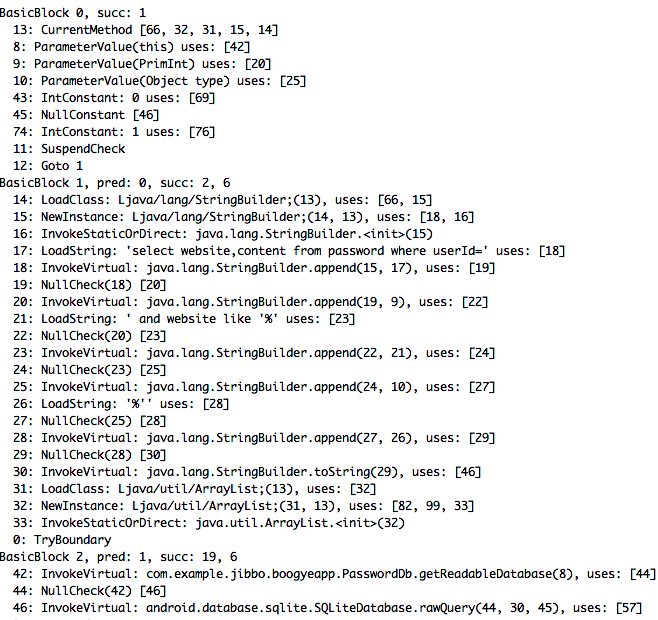
\includegraphics[scale=0.7]{img/query_graph.png}
	\caption{unsafe query example of IR, in its string representation}
    \label{fig:querygraph}
\end{figure}
\newpage
\subsection{Execution of SqlCompSearchInputs}
This algorithm is used to find the source of every StringBuilder. The process starts after the visitor (check section \ref{sec:artist} for reference) finds the \textbf{rawQuery} method: our code checks if the SQL string is composed within a \texttt{StringBuilder} and, if yes, this part of the algorithm is called upon \newline\texttt{StringBuilder.toString()}.\newline Fundamentally, \textbf{SqlCompSearchInputs} computes the backward slice of the before mentioned instruction and while its computing, it also checks the kind of every instruction: if it is a ParamValue, the instruction is added to the tainted set, whilst: if it is instead either LoadString or ConstantValue it stops because they are hard-coded (meaning trusted), otherwise it continues by re-calling itself upon every input of the instructions. Moreover, the algorithm also calls \texttt{SqlCompSearchUse} whenever the instantiation of a StringBuilder is found, this is done to be sure that every usage of the StringBuilder are covered. However, due to its implementation, \emph{Artist} cannot pass arrays to the \textbf{CodeLib}, where the \emph{patchedRawQuery} resides, hence the additions to the tainted set is done by injecting a method, which code resides in the auxiliary library, and passing only the tainted instruction as a parameter to that. Listing \ref{alg:sqlcompsearchinputs} shows the code for this first part of the algorithm.

\begin{algorithm}
\caption{Checking the StringBuilder Backward Slice}
\label{alg:sqlcompsearchinputs}
\begin{algorithmic}[1]
\Procedure{SqlCompSearchInputs}{}
\State $\textit{Node} \gets \text{instruction containing the final query}$
\State $\textit{Graph} \gets \text{The graph containing all the instructions of this block}$
\If{$\text{node \textbf{not in} } \textit{alreadyChecked}}$
	\State $\text{alreadyChecked.add(node)}$
	\If{$\text{node.getKind() \textbf{is}}\textit{NewInstance}}$
		\State $\text{// It's a StringBuilder instantiation}$
		\State $\text{SQlCompSearchUse(node,graph)}$
	\ElsIf{$\text{node.getKind() \textbf{is} }\textit{LoadString or ConstantValue}}$
		\State $\text{// It's safe, we just stop}$
		\State $\text{alreadyChecked.add(node)}$
	\ElsIf{$\text{node.getKind() \textbf{is} }\textit{ParamValue}}$
		\State $\textit{Graph} \gets \text{injectAddToTaintedSet(node)}$
		\State $\text{alreadyChecked.add(node)}$
	\ElsIf{$\text{node.inputCount()} > \text{0}}$
		\State $\text{// It's a NullCheck or an InvokeVirtual}$
		\State $\text{alreadyChecked.add(node)}$
		\For{$i \gets 1 \textrm{ to } node.InputCount()$}
	        \State $\text{SQlCompSearchInputs(node.ChildAt(i),graph)}$
	     \EndFor
	\EndIf
\EndIf
\EndProcedure
\end{algorithmic}
\end{algorithm}


 % All the components are added to the tainted set and this method ends when the algorithm finds all the instantiations of the \textbf{StringBuilder}s themselves, thus calling the second part\footnote{All the hard-coded strings which compose the final sql string are considered safe and not added to the tainted set}. Therefore, \textbf{SqlCompSearchUses} checks that the usages of the string builder and calls \textbf{SqlCompSearchInputs} for every use which wasn't already visited\footnote{The algorithm offers, of course, margins for optimization in both memory and speed, although I preferred to leave the prototype easier to understand to better aid future modifications.}. The tainted set, then gets sent to the support library which code is merged in to the app and that will check at runtime if the query components are tainted and, in the case it might contain an injection, it will prevent its execution. The code of the library can be considered a streamlined version of dynamic analysis. In fact, it scans, at runtime, what is contained in the user inputs and compares it to an hard-coded array of common sql attack vectors. The algorithms that follows are the pseudo-code representation of the above mentioned parts, the library code is omitted for brevity given its simplicity. 

\subsection{Execution of SqlCompSearchUse}
This part of the algorithm gets called when a StringBuilder is instantiated by the call \texttt{NewInstance: java.lang.StringBuilder} and it checks every usage of the builder \texttt{SQlCompSearchInputs}, to ensure that none is omitted. When one of those instruction is found, the first part of the algorithm is called again on that to check whether is a trusted one or untrusted. Listing \ref{alg:sqlcompsearchuse} shows the code for this part of the algorithm.

\begin{algorithm}
\caption{Checking the StringBuilder Usages}
\label{alg:sqlcompsearchuse}
\begin{algorithmic}[1]
\Procedure{SqlCompSearchUse}{}
\State $\textit{Node} \gets \text{instruction containing }\textit{android.database.sqlite.SQLiteDatabase.rawQuery}$
\State $\textit{Graph} \gets \text{The graph containing all the instructions}$
\If{$\text{node \textbf{not in} } \textit{alreadyChecked}}$
	\State $\text{alreadyChecked.add(node)}$
	\If{$\text{node.getName() \textbf{contains not} }\textit{"init"}}$
		\State $\text{SQlCompSearchInputs(node,graph)}$
	\ElsIf{$\text{node.usesCount()} > \text{0}}$
		\State $\text{// It means we still haven't arrived}$
		\State $\text{SQlCompSearchUse(node,graph)}$
	\EndIf
\EndIf
\EndProcedure
\end{algorithmic}
\end{algorithm}

\subsection{The Codelib}
The last piece of the algorithm checks every component sent in the compilation phase by \texttt{SqlCompSearchInputs} and checks at runtime the content of the variables against a static vector of common SQL injection strings. All the tainted components of the query are removed from it before it is executed on the database. Moreover, if no component is flagged as an injection, the algorithm tries to look on the full query for parts that contains at least one of the common injections methods listed in the static vector and, only after nothing is found, the query is executed. The code for this check is trivial due to being mostly only a string comparison. Hence is not reported.

\subsection{Limitations of the Approach}
The hard-coded array contained in \textbf{CodeLib} might represent a point of failure due to the fact that it cannot be comprehensive of all the possible sql injections. However, on Android, prepared statements do not return a resulting cursor and calling the other methods, where safety is achieved by letting the framework compose the query, will require to implement a full-fledged SQL parser. Moreover, despite JSqlParser\footnote{\url{https://github.com/JSQLParser/JSqlParser}}, whose usage has been tested and validated and it was not flexible enough for the goal our prototype needed, the shortage of parsing libraries made impossible, in the constraint of this thesis, to develop a better solution. Further development of this work should tackle this problem and provide a better solution. Escaping is also a viable approach and it was taken into account in the design phase but, using this technique would break the functionalities of all those applications that allow querying directly a database, hence discarded.

\section{Randomness}
The algorithm to replace insecure random usage might seem easy at first. In fact, intuitively, it should be enough to replace the call \texttt{new Random()} with the secure one: \texttt{new SecureRandom()}. However, \emph{ARTist} does not provide a callback to its modules when an instruction of type \texttt{NewInstance} is found. Therefore, in order to patch this, the module needs to wait for the callback that get triggered when the method \texttt{java.util.Random.<init>} is found and then execute a smaller DFS inside the whole block containing the backward slice of this line to find the new instance and replace it. The pseudo-code is as follows:
\begin{algorithm}
\caption{Random patching}\label{euclid}
\begin{algorithmic}[1]
\Procedure{patchRandom}{}
\State $\textit{instruction} \gets \text{instruction containing }\textit{java.util.Random.init}$
\State $\text{randomInstruction} \gets \text{instruction.getBlock().getFirstInstruction()}$
\While{$\text{randomInstruction \textbf{is not} } \textit{null}}$
	\If{$\text{randomInstruction.getKind()} ==  \textit{NewInstance}}$
		\State $\text{debugName} \gets \text{getSignature(randomInstruction)}$
		\If{$\text{debugName contains } \textit{java.util.Random}}$
			\State $\text{brake; // found, go on with the part after this while}$
		\EndIf
	\EndIf
	\State $\text{randomInstruction} \gets \text{randomInstruction.getNext() // will return null at the end}$
\EndWhile
\If{$\text{randomInstruction \textbf{is not} } \textit{null}}$
		\State $\text{injection} \gets \text{injectSafeRandomInstance()}$
		\ForAll{$\text{use} \gets \text{randomInstruction.getUses()}}$
			\State $\text{use} \gets \text{replaceInput(0,injection) // input 0 is the instance of the random}$
		\EndFor
\EndIf
\EndProcedure
\end{algorithmic}
\end{algorithm}

\subsection{Limitations of the Approach}
Given the nature of random number generators, the functionalities offered by an application are not compromised when one is used instead of another\newline ( in the end both should output numbers that look random from the outside), but this holds true only when swapping one algorithm for a more secure one. As already explained in section \ref{sec:randominvestigation}, this is the case in our algorithm and, although there is no perceivable difference between the output of the two when used inside an application, it should also hold true from a user perspective. In fact, unless a developer is exploiting the weaknesses of the class Random explicitly, an end user should not notice any difference in the behavior of the program. Moreover, since it can be assumed that the everyday user cannot tell the difference between two numbers obtained from two different generators, the only way they can notice the algorithm swap is when a significant decrease in performance takes place. On this regard, the documentation published by Oracle only states that \texttt{SecureRandom} has to wait, before returning a value, until enough entropy is available and the official Android one does not mention differences in execution speed between the afore-mentioned class and \texttt{Random}. For this purpose, I developed an app, which code is available on Github\footnote{https://www.github.com/jibbo/master\_thesis}, to test their performances. The app was executed multiple times on a low-end device such as the Kindle Fire (7 inches model, 2017 version), which has a 1.3Ghz arm quad-core processor from Mediatek and it has been rebooted before each execution of the test. \texttt{Random} was generating an Integer number instantly, whilst \texttt{SecureRandom} took, on average, 1ms. Although this test needs to be run on a larger scale, it suggests that on similar hardware there is a small decrease of performance. However, a 1ms delay is not perceivable by users, hence replacing Randomness can be considered a safe patch which only improves security.

\section{Hashing}
As already discussed in chapter \ref{ch:investigation}, MD5 and SHA1 have been proven to be broken. However, they are still widespread among app developers to verify the integrity of packages or for other needs. What the module does in this case, is replacing the algorithm name when invoking the instance of \texttt{MessageDigest} with SHA-256.

\begin{algorithm}
\caption{Hashing patching}\label{euclid}
\begin{algorithmic}[1]
\Procedure{patchHash}{}
\State $\textit{instruction} \gets \text{instruction containing }\textit{java.security.MessageDigest.getInstance}$
\State $\textit{safeAlgName} \gets \text{"SHA-256"}$
\State $\text{instruction.InputAt(1)} \gets \text{safeAlgName}$
\EndProcedure
\end{algorithmic}
\end{algorithm}

\subsection{Limitations of the Approach}
Despite the simplicity of the modification, changing the algorithm used for hashing is very delicate and might break functionality. This contrasts the third characteristic of an ideal tool and this is why this patch is considered "Risky". In particular, the dysfunction happens all the times that an external part of an application architecture, which \emph{DevArtist} is unaware of, does not support the new hashing algorithm. For example: an application that downloads and verifies an add-on via MD5 and, if the hash matches with the one specified by the server, it enables the add-on, otherwise it triggers the download again. In this case, the proposed solution breaks the integrity check due to the algorithm mismatch between application and server, producing an unusable application by keeping it in the verification (plus download) loop for a long time and eventually making it crash as soon as the maximum amount of resources allocated for the process ends.

\section{Debating the Usefulness of DevArtist}
In the previous chapter are described the reasons why patching these vulnerabilities is a necessity, but it is worth to mention that not all the signatures found by \emph{DevArtist} can be exploitable by an attacker, such as, for example, it can be a SQLi injection in a query which is never executed. Moreover, the proposed fixes cannot patch vulnerabilities completely in all the cases and this, united with the example just mentioned and the fact that risky patches reduces the functionality of an app, question the usefulness of \emph{DevArtist}. However, as already mentioned in this work, it is important to see \emph{DevArtist} in its context, which is the one of a prototype not yet suitable for the masses but only for security focused environments and privacy concerned experimenters. Therefore, for this niche, hardening the most of a system is not only important but better due to the fact that it improves the overall security by making the whole environment less prone to attacks. In addition, project such as F-Droid\footnote{\url{https://f-droid.org}}, which is an open-source market for apps, show that patches which break application functionalities do not limit considerably the number of this particular subset of users, due to the fact that they are accustomed to use less apps, provided that the ones that work are perceived as more secure.

 

    \chapter{Evaluation}
\label{ch:evaluation}
The goal of this evaluation is to shed light over the success rate of \emph{DevArtist}. Therefore, a similar process to the one described in chapter \ref{sc:preliminaryanalysis} was used and, in fact, it required to install \emph{DevArtistGui} into the device and instruct Monkey Troop on the same subset of apps taken into consideration before. However, this time, every patching solution has been run separately to increase the granularity of the results and the steps executed by the testing tool also tried to emulate a person using the app. In this way, the test was able to check whether a target app was crashing only after the patches were applied.

\subsubsection{Commands for Monkey Troop}
The most visible change in the steps that follow, from the commands executed by Monkey Troop in chapter \ref{sc:preliminaryanalysis}, is represented by the attempt to emulate the usage of the app from a user. However, the capabilities of this automated tester are limited to executing taps at random coordinates of the screen, due to the fact that it does not provide any API to choose where or how to interact with apps. Although this simulation cannot be considered as precise as a real person who taps in the right parts of the screen, it is the best possibility with the available tools.
% of a user wasachieved by generating a random set of coordinates within the resolution of the screen and letting the tester perform those before and after instrumenting a target app.

\begin{enumerate}
	\item{Download an app from the Play Store}
	\item{Install the app on the device(s)}
	\item{Run the app}
	\item{Perform random taps in the app}
	\item{Close the App}
	\item{Start ArtistGUI}
	\item{Instrument the app}
	\item{Run the instrumented App}
	\item{Perform the same random taps in the instrumented app}
	\item{Repeat from 1 with another app from the list}
\end{enumerate}

\subsubsection{The List of Apps}
Following the goal of this work, it was necessary to take into consideration the same set of apps described in chapter \ref{sc:preliminaryanalysis}. It allowed not only to compute how accurate the patching was, but also to check whether \emph{Artist} was suffering of a lower success rate in instrumenting a target app than before my module was applied.   

\section{Results}
Despite the patch for every signature is injected every time a vulnerability is found statically, given the dynamic phase of \emph{DevArtist}, I considered as patched only the logs produced during runtime. Therefore, is it possible that the random taps generated by Monkey Troop couldn't reach all the points of the app where the vulnerable signatures are called, thus showing low numbers in the interested column. Furthermore, all apps that could not be instrumented or crashed after instrumentation (over the total 492) are considered failures. In addition to the data presented in table \ref{tab:evaluation}, the reader should know that \emph{Artist} alone, without any of my code, failed in 33 cases, having a success rate of 85,40\%.
\vspace{1.5cm}
\begin{table}[H]
	\centering
	\begin{tabular}{|c|c|c|c|c|}
		\hline
		Patch & Times Found & Successes & Failures & Unknown State\\
		% \hline
		% Random & 261 & 110 & 111+80 & 151\\
		% \hline
		% rawQuery & 296 & 108 & 45+196 & 161\\
		% \hline
		% Hashing & 308 & 210 & 55+86 & 98\\
		% \hline
		Random & 261 & 110 & 111 & 231\\
		\hline
		rawQuery & 296 & 108 & 45 & 196\\
		\hline
		Hashing & 308 & 210 & 55 & 184\\
		\hline
	\end{tabular}
	% \begin{tabular}{|c|c|}
	% 	\hline
	% 	Patch & Failures\\
	% 	\hline
	% 	Random & 111 \\
	% 	\hline
	% 	rawQuery  & 45 \\
	% 	\hline
	% 	Hashing & 55 \\
	% 	\hline
	% \end{tabular}
	% \newline\newline\newline
	% \begin{tabular}{|c|c|}
	% 	\hline
	% 	Patch & Unknown State\\
	% 	\hline
	% 	Random & 151 \\
	% 	\hline
	% 	rawQuery  & 161 \\
	% 	\hline
	% 	Hashing & 98 \\
	% 	\hline
	% \end{tabular}
	\caption{Results}
	\label{tab:evaluation}
\end{table}
\newpage
\section{Interpretation}
The most interesting result in the data presented in table \ref{tab:evaluation}, is that insecure randomness has been patched in the 42,14\% of the time, showing that changing the random algorithm is more delicate than predicted. The reason behind this finding might be that developers indeed know when to use which algorithm and, in fact, there is a subset of apps which are internally using both \texttt{Random} and \texttt{SecureRandom}, as shown in table \ref{tb:respreliminary} (chapter \ref{ch:investigation}). Patching the \texttt{rawQuery} method is successful, instead, in more than 36,48\% of the times, making instrumentation of the applications crash only 12 times more than \emph{Artist} itself, which is a good result given the amount of code needed for the patch. It is also interesting to find the patch of broken hashing functions to be less risky than imagined. In fact, this patch worked more than 68,18\% of the times, with a failure rate of only 4,5\% more than \emph{Artist} itself (11,2\% vs 6,7\%). This exceptional data suggests that developers need to be more careful when using hashing functions and not only decide to use a secure one, but also to verify its correct usage. It is important to note that, as already stated in the previous section, logs for successful patches are generated at runtime only when the patching code is triggered. Hence, since that code is injected before each vulnerable signature is called, the number of successful patches could have increased if Monkey Troop would have performed a set of taps targeting all the specific executions paths of the apps containing the vulnerable signatures. This is also the main reason behind the unknown state table, all those apps might have been successfully patched or not but until they are manually executed and every one of their execution paths is taken their state cannot be determined.
However, if collected, more than 49,47\% of the apps were successfully patched without decrease in app functionalities.

% It is interesting to note that the easiest patch, the one using \texttt{Random} instead of \texttt{SecureRandom}, was successfully applied only in the 82,15\% of the apps. Moreover, patching the \texttt{rawQuery} method without experiencing crashes or instrumentation failures was successfull 
% The numbers presented above picture a different reality than the one imagined in chapter \ref{ch:devartist}. In fact, the patch with the lowest number of failures is the Hashing one, making it the less "risky" patch.

    \chapter{Future Work}
\label{ch:futurework}
Given that the focus of this thesis in providing a novel and compiler-based tool to improve security, its state is prototypical and far from being optimal. However, it provides a solid base for further development in the area, which can start from what is here presented.

\section{Support for Additional Platforms}
Currently, \emph{DevArtist} is available only on arm processors for Android 7 Nougat, but it can be easily shipped for any Android platform, where \emph{Artist} is available, by re-compiling dex2oat within all the other Android versions and publish the packages on the Google Play Store. This would enable more people to benefit from this work.

\section{Optimizations}
The current algorithm which checks for SQL Injections is using a static vector for comparison. This issue should be addressed to substantially improve the accuracy of detection and reliability of the patching. The goal can be achieved by implementing a full-fledged SQL parser in Java which checks and enforce, at runtime, the constraints of the SQL query. Moreover, the current algorithm which detects the non hard-coded parts of the query string, at the compiler-level, could be optimized to increase its speed and lower its memory footprint.

\section{Discarding Root as Requirement}
\label{sc:discardroot}
Root is mandatory due to the fact that the on-device OAT file produced by the original application has to be replaced with the one compiled within our system and its location is protected by Android. However, a solution to this problem is provided in \cite{boxify}, which enables a light-weight but full-fledged sandboxing system without relying on OS modifications or root. In particular, it re-implements parts of the Android middleware in the sandbox and virtualize parts of the privileged filesystem, thus enabling apps to be installed without being root. Alternatively, as discussed in \ref{sc:deploy}, a custom ROM could replace the original dex2oat with our one and, by being a system app with higher privileges, it does not require root permission to install app. Projects such as CopperOS and LineageOS, could advertise this move as a way to improve the overall security, whilst \emph{DevArtist} would benefit by gaining more eyes (and hopefully improvement) on its source-code.

\section{Extensions}
One helpful extension of \emph{DevArtist} could be the possibility to choose between which of the three patches a user wants to apply on a per-app basis. This would greatly improve the usability for experimenters that would like to exclude risky patches and only use the safe ones.\newline
In addition, a system as \emph{DevArtist} can be used as a base to further improve security. In fact, by extending the auxiliary library it would be interesting to check at runtime if strings contained in variables are passwords and check if they are stored unencrypted. If that is the case, the project could provide "transparent" encryption for passwords stored in SharedPreferences, Files, Databases and so on, without requiring any modification from a developer.\newline
However, one of the best extensions the system might support is the ability to define a sort of \enquote{policy} for each vulnerability, by declaring the signature of a vulnerable method, and including in it also the way to patch it. This approach would offer to developers of companies to create custom policies for their own code and it would enable to speed up the code reviewing process.\newline
Moreover, this could even be extended more and create something similar to PatchDroid\cite{patchdroid}: given a repository for every vulnerability and platform, \emph{DevArtistGUI} could send to it information about a target app and the device on which it is running and receive back the proper version of \emph{dex2oat} and \emph{Codelib} to patch the vulnerabilities exposed by the selected app.\newline


\chapter{Conclusion}
The first contribution of this work used the empirical data in chapter \ref{ch:investigation} to show that developers still code insecurely, finding that unsafe randomness, obsolete hashing functions and insecure methods to query databases are still widely used on the top apps of Android's Play Store. This thesis also proposed a few threat models for the before-mentioned issues, to help understanding the necessity of the second contribution: a patching prototype described in chapter \ref{ch:devartist}. This solution's novelty manifests in the usage of the new Android on-device compiler and it also shows its advantages for the end user in respect to already existing tools. Despite the prototypical stage of the proposed system, it manages to achieve two of the main characteristics of an ideal tool and the automated tests, executed in chapter \ref{ch:evaluation}, suggest the usefulness of \emph{DevArtist} in the fight against malware. In fact, the evaluation's result are promising and hint that for the 49\% of the analyzed apps, the system reduces their attack surface while keeping them functional. Moreover, in contrast to expectation, these results also showed that changing the hashing algorithm in applications is safer than replacing the underlaying randomness, making the latter more of a risky patch than the former. Although \emph{Monkey Troop} enabled to run tests on a larger amount of apps than manually possible, which incremented the scale of the investigation, it also limited the precision of the results and other further findings, showing that there is a need for more research and development in the area. In conclusion, this thesis evaluated the need of patching vulnerabilities left open by developers, suggests a partial solution by creating a prototype addressing SQL Injections, unsafe Random usage and obsolete Hash Functions, thus showing, through evaluation, that patching those vulnerabilities can be done effectively at a compiler-level and increasing the overall security of a device.

%However, the success rate and other findings could have been more precise if \emph{Monkey Troop}, even tough it enabled to run tests on a larger amount of apps than manually possible, was capable to reach every execution path, thus requiring further development. In conclusion, final users who have root permissions can already harden the security of their devices by installing DevArtistGUI or wait for a Custom ROM which ships with it.






     
    \chapter*{Acknowledgements}
\thispagestyle{empty}

I would like to thank my advisor Oliver for its great support and understanding, whenever we talked about a problem I was encountering, he always provided help and insights on how to go investigate deeper.\newline I would also like to thank Professor Micheal Backes and Fabio Massacci to take the time to review this work.\newline A special thank goes to my mum Melina, my aunt Nadia but also to my grand parents Angela and Emilio.\newline Big thanks also to all my friends who supported me for this three years, particular mention goes to: \'Abris Nagy, Istev\'an Seres, Riccardo Spadi, Francesco La Tegola, Artem Perlov and Roberto Zen. You guys rock!\newline Thanks and still many thanks to DUIR for their unconditional support during the whole time abroad: thanks to all of you guys for not replacing me, it meat a lot to me.\newline Huge thanks to the company which I worked for during the study on this work: Backes-SRT and in particular I would like to thank Sven Obser and Fabian Bendun, they provided a relaxing environment and an incredible support.\newline A special mention and thank goes to Sara Tacchetto for being at my side and to be always there in the darkest moments. Also, thanks for reading this work (and all the related powerpoints and talks) countless times.\newline There are a lot more people I should thank for accompanying me in this experience, but they would be too many to put here: you know who you are and you are all amazing people.
  \appendix
    \chapter{Auxiliary data}
I list and collect all the raw data, which is previously referenced in this work, as a reference for the reader who wants to perform further investigations.

\begin{figure}
	\centering
	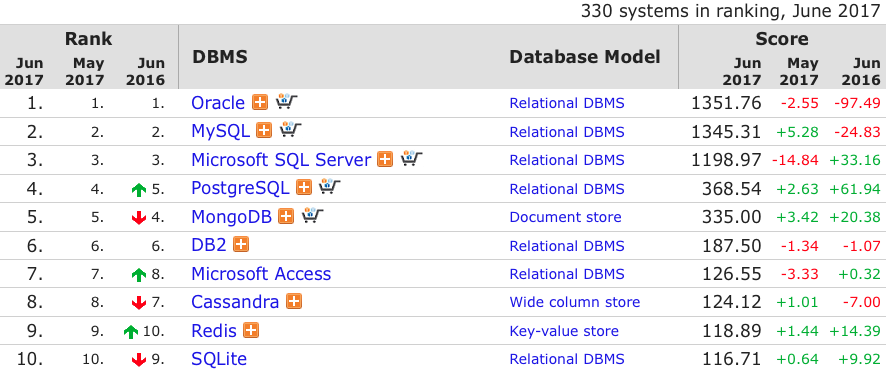
\includegraphics[scale=0.5]{img/dbmarketshare.png}
	\caption{Database Marketshare: Snapshot as of 2017-06-24}
    \label{appendix:dbmarketshare}
\end{figure}

\section{List of categories}
\label{appendix:categorieslist}
\begin{verbatim}
BOOKS_AND_REFERENCE
BUSINESS
COMICS
COMMUNICATION
EDUCATION
ENTERTAINMENT
FAMILY
FAMILY_AGE_RANGE3
FAMILY_ACTION
FAMILY_BRAINGAMES
FAMILY_CREATE
FAMILY_EDUCATION
FAMILY_MUSICVIDEO
FAMILY_PRETEND
FINANCE
GAME_ACTION
GAME_ADVENTURE
GAME_ARCADE
GAME_BOARD
GAME_CARD
GAME_CASINO
GAME_CASUAL
GAME_EDUCATIONAL
GAME_MUSIC
GAME_PUZZLE
GAME_ROLE_PLAYING
GAME_SPORTS
GAME_STRATEGY
GAME_TRIVIA
GAME_WORD
HEALTH_AND_FITNESS
LIBRARIES_AND_DEMO
LIFESTYLE
MEDIA_AND_VIDEO
MEDICAL
MUSIC_AND_AUDIO
NEWS_AND_MAGAZINES
PERSONALIZATION
PHOTOGRAPHY
PRODUCTIVITY
SHOPPING
SOCIAL
SPORTS
TOOLS
TRANSPORTATION
TRAVEL_AND_LOCAL
WEATHER
\end{verbatim}

\section{List of apps}
\label{appendix:appslist}
\begin{verbatim}
    ak.alizandro.smartaudiobookplayer
    androbros.com.wordfit
    app.hungnv.com.hdwallpaper
    ar.com.soodex.ahorcado
    at.appingo.pillreminder
    at.tomtasche.reader
    batalsoft.band.live.rock
    batalsoft.drumsolohd
    batalsoft.drumsolohd.rock
    batalsoft.piano.solo.hd
    beemoov.amoursucre.android
    biz.bookdesign.librivox
    biz.neoline.neomult
    br.com.rodrigokolb.realbass
    br.com.rodrigokolb.realdrum
    br.com.rodrigokolb.tabla
    by.ai91.lyfoes
    cc.dict.dictcc
    cellfish.spidermanlwp
    cgeo.geocaching
    ch.admin.meteoswiss
    ch.publisheria.bring
    ch.threema.qrscannerplugin
    chessfriends.online.chess
    com.aadhk.time
    com.abaenglish.videoclass
    com.abbyy.mobile.lingvo.market
    com.adpog.diary
    com.advancedprocessmanager
    com.aerilys.acr.android
    com.agt.smokerstop
    com.airwatch.androidagent
    com.airwatch.email
    com.aitype.android
    com.alensw.PicFolder
    com.alphablind.nabu
    com.amalpro.ta3alom_almaniya
    com.amazon.buyvip
    com.amazon.mp3
    com.amazon.mShop.android.shopping
    com.ancestry.android.apps.ancestry
    com.androbaby.voicechanger
    com.androbros.puzzle2048eng
    com.androidrocker.callblocker
    com.anghami
    com.anyoption.android.app
    com.apalon.ringtones
    com.apalon.wallpapers
    com.app.studio.mp3player
    com.app.studio.voicerecord
    com.app_hockenheimgp.layout
    com.appsvolume.mostPopularRingtonesFree
    com.appxy.tinyscanner
    com.apusapps.launcher
    com.arabdict.dictionary
    com.arcsys.tictactoe
    com.arkiaapps.pouegg
    com.asgardsoft.words
    com.atistudios.italk.de
    com.atistudios.italk.es
    com.audials
    com.augmentra.viewranger.android
    com.avg.cleaner
    com.aviary.android.feather.plugins.borders.free
    com.aviary.android.feather.plugins.stickers.free_stickers
    com.avira.android
    com.baviux.voicechanger.kids
    com.berniiiiiiii.wortspiel
    com.binteraktive.kniffel.live
    com.binteraktive.madnlight
    com.bluefirereader
    com.booking
    com.brainium.spiderfree
    com.bzzzapp
    com.calfordcn.gu
    com.cantecegradinita.ro.app
    com.CartoonImage.DIY
    com.cashquizz.cashquizz
    com.catple.wallpapers
    com.chatous.pointblank
    com.chess
    com.chsoftware.regenvorschau
    com.cisco.anyconnect.vpn.android.avf
    com.cmcm.lite
    com.com2us.smon.normal.freefull.google.kr.android.common
    com.commerzbank.photoTAN
    com.cootek.smartinputv5
    com.crimsonpine.stayinline
    com.cutegirl.animegirl.hdwallpaper
    com.daf.archanoide
    com.damiapp.softdatacable
    com.darkhorse.digital
    com.dataviz.docstogo
    com.dawidkiljan.bplogger
    com.db.pbc.phototan.db
    com.db.pbc.phototan.nb
    com.dccomics.comics
    com.developandroid.android.animals
    com.dianxinos.dxbs
    com.djinnworks.StickCliffDiving.lite
    com.dokdoapps.mybabymusicboxes
    com.dokdoapps.mybabypiano
    com.dragonplay.liveholdempro
    com.dragonplay.slotcity
    com.drillyapps.babydaybook
    com.droidhen.game.poker
    com.duapps.antivirus
    com.duapps.cleaner
    com.duckduckgo.mobile.android
    com.duolingo
    com.e3games.plus2048
    com.e3games.wordsearchgerman
    com.educ8s.triviaquiz2015
    com.ehraman.anime.girl.live.Wallpaper
    com.eisterhues_media_2
    com.eliferun.music
    com.emoji.ikeyboard
    com.energysh.drawshow
    com.enlightment.appslocker
    com.enrasoft.scratchthat.logoquiz
    com.estrongs.chromecast
    com.evernote
    com.eyewind.colorfit.animal_kingdom
    com.eyewind.colorfit.mandala
    com.famousbluemedia.yokee
    com.fatsecret.android
    com.food.calories
    com.fortafygames.colorswitch
    com.free.apps.truth.or.dare
    com.ftbpro.app
    com.g6677.android.phairsalon
    com.game.wer.wird.millionaer
    com.gamelikeapp.carbrands
    com.gamesforfriends.icomania
    com.gamma.scan
    com.gemego.klondikefree
    com.ghstudios.android.mhgendatabase
    com.goldenballgames.islandbubbleshooter
    com.google.android.apps.books
    com.google.android.apps.magazines
    com.google.android.stardroid
    com.google.android.street
    com.google.zxing.client.android
    com.graphicalize.comicize.app
    com.graphics.logodesign
    com.groesel.emojiwort
    com.hardgrnd.lineup11
    com.hasbro.tf360appstore
    com.hearing.healthcare.siemens.touchcontrol
    com.herman.ringtone
    com.hssn.anatomyfree
    com.iconology.comics
    com.ideashower.readitlater.pro
    com.idmobile.deutschlandmeteo
    com.igg.clashoflords2
    com.ikeyboard.emoji.emojione
    com.ikeyboard.theme.anchor_galaxy
    com.ikeyboard.theme.black_white
    com.ikeyboard.theme.BlackandSliver
    com.ikeyboard.theme.golden_bow
    com.ikeyboard.theme.hellfire
    com.ikeyboard.theme.NeonLight
    com.ing.diba.smartsecure2
    com.intsig.BCRLite
    com.intsig.camscanner
    com.itipton.germanverbs
    com.jappy.mobileMessenger
    com.jb.gokeyboard
    com.jb.gokeyboard.sticker.emoticon
    com.jb.zcamera
    com.joeware.android.gpulumera
    com.joeykrim.rootcheck
    com.jrummy.apps.google.play.api
    com.kaspersky.qrscanner
    com.kathleenOswald.solitaireGooglePlay
    com.kauf.sticker.funfacechangerproeffects
    com.kdanmobile.android.pdfreader.google.pad
    com.keramidas.MarketUpdateHelper
    com.kidsthree.babyfashiontailor
    com.kii.safe
    com.kiragames.unblockmefree
    com.kt.telephone
    com.lalasoft.boyutluduvar
    com.lbrc.PeriodCalendar
    com.lenovo.anyshare.gps
    com.lexa.fakegps
    com.lochmann.ninemenmorris
    com.lubosmikusiak.articuli.derdiedas
    com.lulo.scrabble.classicwords
    com.macropinch.swan
    com.magine.aliceoid
    com.magnetic.openmaps
    com.marvel.comics
    com.masarat.salati
    com.matz.dwdwetter
    com.maxxt.pcradio
    com.mdv.RheinbahnCompanion
    com.medicalgroupsoft.medical.directorymedtermsmultilang.free
    com.melimots.WordSearch
    com.mg.android.free
    com.microsoft.rdc.android
    com.microsoft.skydrive
    com.microsoft.windowsintune.companyportal
    com.miniclip.agar.io
    com.miniclip.animalshelter
    com.miniclip.eightballpool
    com.miniclip.hockeystars
    com.miniclip.soccerstars
    com.mobile.bizo.slowmotion
    com.mobilecreatures.drinkwater
    com.mobilityware.solitaire
    com.mobilityware.spider
    com.mobilplug.lovetest
    com.mobisystems.editor.office_with_reg
    com.mobisystems.fileman
    com.mobisystems.ubreader_west
    com.mobvantage.CashForApps
    com.monks.praxis_app.activitys
    com.monotype.android.font.flipfont.qisifont.Sweetie
    com.monotype.android.font.free.fifty6
    com.monster.android.Views
    com.mousemobile.explorationcraft
    com.movinapp.dict.ende.free
    com.msi.logogame
    com.mtapps.quiz.football_clubs_quiz
    com.mustafademir.xylophone_for_kids
    com.mxtech.ffmpeg.v6
    com.mxtech.ffmpeg.v6_vfp
    com.myfitnesspal.android
    com.myyearbook.m
    com.netbiscuits.adac
    com.netflix.mediaclient
    com.netmarble.momag
    com.netqin.ps
    com.nighp.babytracker_android
    com.nike.pass.root
    com.ninetyfour.degrees.app
    com.no_magic.kennzeichen_d
    com.nullapp.minipiano
    com.obproject.de
    com.ogqcorp.bgh
    com.opera.mini.native
    com.optimesoftware.hangman.free
    com.optimesoftware.tictactoe.free
    com.panaceasupplies.android.reader
    com.pescapps.kidspaint
    com.photoedit.photocollage
    com.pinkpointer.crosswords
    com.piriform.ccleaner
    com.poker.clubs.wallpapers.cute.anime.girl
    com.popularapp.periodcalendar
    com.popularapp.sevenmins
    com.postillon
    com.priotecs.MoneyControl
    com.progimax.airhorn.free
    com.qisiemoji.inputmethod
    com.qrcodereader
    com.quantrity.anttester
    com.quelaba.sopaletras
    com.quizapp.multitable
    com.quvideo.xiaoying
    com.radiosonline.deutschefmradio
    com.rarlab.rar
    com.readfy.app
    com.readly.client
    com.riffsy.FBMGIFApp
    com.rookiestudio.perfectviewer
    com.rt.mobile.english
    com.ruanshaomin.game
    com.rvappstudios.magnifyingglass
    com.sal.hdplaytubevideo
    com.sgiggle.production
    com.sgmcpe.mc1
    com.shadoweinhorn.messenger
    com.sinyee.babybus.babyhospital
    com.sinyee.babybus.birthdayparty
    com.sinyee.babybus.chef
    com.sinyee.babybus.dj
    com.sinyee.babybus.magichouse
    com.sinyee.babybus.recommendInter
    com.sinyee.babybus.seaworld
    com.sinyee.babybus.toilet
    com.sinyee.babybus.truck
    com.sinyee.babybus.wobunanguo
    com.sirma.mobile.bible.android
    com.skype.raider
    com.sleekbit.dormi
    com.smoqgames.fopenpack
    com.smsrobot.period
    com.smule.autorap
    com.sofascore.results
    com.sonos.acr
    com.sonyericsson.trackid
    com.Splitwise.SplitwiseMobile
    com.starfinanz.mobile.android.dkbpushtan
    com.statussprueche
    com.surpax.ledflashlight.panel
    com.suvorov.de_en
    com.sweefitstudios.drawtattoo
    com.sytel.de.galade
    com.taplane.triviaquiz
    com.tapsarena.find
    com.teamlava.matchbakery55
    com.tekaris.richtigtanken
    com.tencent.mm
    com.thaidevelopers.junglebubble
    com.tinymission.dailyworkoutsfree
    com.tippingcanoe.mydealz
    com.tippingcanoe.urlaubspiraten
    com.tmarki.comics
    com.tnature3.Mahjong
    com.tobiapps.android_100floors_guide
    com.tplink.tether
    com.ubimet.uwr
    com.UCMobile.intl
    com.uefa.ucl
    com.upp.drawcartoons
    com.upp.illusionsdrawing
    com.urbandroid.lux
    com.vertaler.deen
    com.vertaler.deit
    com.viewer.comicscreen
    com.visualit.tubeLondonCity
    com.vladlee.easyblacklist
    com.vysionapps.faceswap
    com.weheartit
    com.wetter.androidclient
    com.wetter.radar
    com.whatsapp
    com.wikihow.wikihowapp
    com.winzip.android
    com.wlingua.curso
    com.wordsmobile.musichero
    com.workshophk.t2rcmecy
    com.xing.android
    com.xodo.pdf.reader
    com.xoopsoft.apps.bundesligatwo.free
    com.ysb.esh
    com.yx.boxinghero
    com.zentertain.photoeditor
    coml.macromassive.babytooth.app
    couchDev.tools.DocxParser
    cz.aponia.bor3
    cz.aponia.bor3.offlinemaps
    de.adac.android.autodatenbank
    de.aerzteblatt
    de.aktiwir.aktibmi
    de.amedicksommer.meinbaby.speyer
    de.appfiction.yocutiegoogle
    de.avm.android.myfritz
    de.barcoo.android
    de.betaapps.bruttonetto
    de.bfv.android
    de.buhl.wisogehalt
    de.casparwre.insult
    de.cellular.stern
    de.dealdoktor.app
    de.deltacity.android.blutspende
    de.deutscherfahrschulverlag.fsc
    de.dfbmedien.egmmobil
    de.dieEinsteiger.Liniennetze
    de.dkb.portalapp
    de.embryotox
    de.faplino
    de.finanzen.net
    de.finanzen100.currencyconverter
    de.flame.dartcounter
    de.flowfwd.supzit
    de.focus.topnews
    de.gmx.mobile.android.mail
    de.habanero.quizoid
    de.hansecom.htd.android
    de.heute.mobile
    de.ing_diba.kontostand
    de.jkg.einkaufsliste
    de.kicktipp.mbookmark
    de.kividoo.vod
    de.komoot.android
    de.lotum.whatsinthefoto.de
    de.lotum.whatsinthefoto.us
    de.marktjagd.android
    de.mcoins.applike
    de.md.meinmd
    de.mobile.android.app
    de.nordbayern.news.live
    de.onvista.onvista
    de.osogo.gehaltsrechner
    de.pappermint.notfallsani
    de.qvc
    de.rs.besserwisser
    de.schildbach.oeffi
    de.sellfisch.android.wwr
    de.sport1.darts
    de.sport1.radio
    de.sueddeutsche
    de.swm.mvgfahrinfo.muenchen
    de.theorie24.fs.mofa
    de.trimexa.urlaubsguru
    de.tvspielfilm
    de.unister.boersennews
    de.wdr.einslive
    de.web.mobile.android.mail
    de.winsim.servicewelt
    de.wucop.quiz
    de.zalando.mobile
    de.zeit.online
    deezer.android.app
    dimala.trueordare.free
    example.matharithmetics
    flipboard.app
    game2048.b2048game.twozerofoureight2048.game
    ginlemon.smartlauncher.extratool
    ginlemon.smartlauncher.notifier
    hu.appcoder.solitaire
    ilmfinity.evocreoFree.main.android
    info.marlan.is24
    jp.naver.line.android
    jpark.AOS5
    kr.co.smartstudy.pinkfongtv_android_googlemarket
    lemmingsatwork.quiz
    logos.quiz.companies.game
    mangatutorial.drawanime
    mbinc12.mb32b
    me.pou.app
    media.mp3.audio.musicplayer
    media.music.musicplayer.mp3player
    mg.locations.track5
    midasapps.fingertwister
    minecraftguns.mod.gunsmodmcpe
    mobi.infolife.ezweather.widget.clockandweather
    mobi.mgeek.TunnyBrowser
    mobil.ardtext
    mp3.cutter.ringtone.maker.trimmer
    mz.sudoku
    net.faz.FAZ
    net.fussballtransfers.mobile
    net.osmand
    net.peakgames.mobile.android.tavlaplus.android
    net.peakgames.OkeyPlus
    net.skoobe.reader
    net.skyscanner.android.main
    net.traveldeals24.main
    net.tsapps.topdeals
    net.zedge.android
    nextapp.fx
    org.anddev.android.solfa_lite
    org.blitzortung.lightning.tracker.app
    org.dtalpen.athantimetr
    org.geometerplus.zlibrary.ui.android
    org.kde.necessitas.ministro
    org.opencv.engine
    org.withouthat.acalendar
    pl.com.smoktunowicz.ufd
    pl.lukok.draughts
    pl.nenter.app.flashlightgalaxys5
    pl.netaddict.hworld
    rschrenk.kinderlieder
    ru.ok.android
    se.appfamily.animalpianofree
    se.feomedia.quizkampen.de.lite
    skat.am.stammtisch.frei
    spin.the.bottle.truth.or.dare
    theme.ice.wolf.game.thrones
    tr.com.alyaka.alper.drum2
    tr.com.alyaka.alper.toddlerstrombone
    tv.arte.plus7
    tv.viva.charts
    vcam.dk.DeutschNachrichtenZeitungen
    video.player.audio.player.music
    vsin.t16_funny_photo
    wp.wattpad
    ws.letras
    yourapp24.android.tools.alice_lite
\end{verbatim}
 
% \includepdf[fitpaper,pages={1-}]{found.pdf} 
% \includepdf[fitpaper, pages={1-}]{unfound.pdf}

  \bibliographystyle{unsrt}
  \bibliography{bibliography}
\end{document}
